\chapter{%Sensitivity analysis of optimal investment times
Simulation study of the optimal investment times}
\label{chapter:stoptime}



%%%%%%%%%%%%%%%%%%%%%%%%%%%%%%%%%%%%%%%%%%%%%%%%%%%%%%%%%%%%%%%%%%%%%%%%
\section{Introduction}
\label{section:stoptime_intro}

In this chapter we analyse the optimal times to invest regarding the three different models developed on previous chapters, using simulation analysis. Following the (usual) studies performed concerning real options, only the influences of the demand level and market's uncertainty are studied.

%First, we will analyse some relevant measures - such as estimated mean, median and standard deviation - concerning the behaviour of optimal investment times with different initial demand values.
Regarding the following simulations performed, the optimal stopping times are calculated on different ways.
For Chapters \ref{chapter:1} and \ref{chapter:2} (and accordingly to the diagrams presented on Figures \ref{1_time} and \ref{2_time}, respectively) there is a single optimal investment time which is calculated considering as initial instant the time at which the innovation breakthrough takes place.
On Chapter \ref{chapter:3} (and accordingly to the diagram on Figure \ref{3_time}), we have two optimal investment times: the optimal time to enter the market with the new product, $\tau_1$, and the optimal time to abandon the old product, $\tau_2$, considering as initial instant the time when the new product is adopted, that is $\tau_1$. Therefore, if one wants to know the estimated optimal time when a firm should abandon the old product after its entrance in the market, one should sum $\tau_1$ and $\tau_2$, for example.


We first consider, by analysing, statistical measures of the simulated series (in particular: mean, median and standard deviation), we study the influence of initial demand values on optimal investing times.
Secondly, we analyse how the estimated mean of optimal investment times behaves with volatility and assess its relation with changes  either on the associated threshold value or optimal capacity level.

On Appendix \ref{chapter:appendixVectors} are presented the most important functions implemented in \texttt{Mathematica}.

\section{Sensitivity of the optimal investment times w.r.t. initial demand value, $x_0$}
\label{section:x0}

\subsubsection{Methodology}


%%%%%%%%%%%%%%%%%%%%%%%%%%%%%%%%%%%%%%
We analyse model by model, initially fixing relevant parameters to the considered situation, with the exception of the initial point $x_0$ - which is changed.
Considering the values fixed on previous comparative sections, in particular of Chapter \ref{chapter:3}, with the exception of the volatility, which we increased to $\sigma=0.1$, the main procedure followed is described on the diagram hereunder:

\vspace{0.5cm}
\begin{tikzpicture}[
level 1/.style={sibling distance=10cm},
edge from parent/.style={->,draw},
>=latex]

% root of the the initial tree, level 1

\node[root] (r) {\textbf{1.} Fix parameters of interest:
}
% The first level, as children of the initial tree
child {node[level 2] (c1) {\textbf{Chapters \ref{chapter:1} and \ref{chapter:2}}}}
child {node[level 2] (c2) {\textbf{Chapter \ref{chapter:3}}}};

%\begin{scope}[every node/.style={root}] 
%\node[above of = r , xshift=-30pt] (svc0) {svc\_top=0};
%\node[above of = r , xshift=30pt] (svc1) {svc\_top=1};
%\end{scope}

% The second level, relatively positioned nodes
\begin{scope}[every node/.style={level 3}]
\node [below of = c1, xshift=2.5cm, yshift=-3cm] (c11) 
{
	$\bullet$ Xstep=0.0002\\
	$\bullet$ Xmin=0.0002\\
	$\bullet$ Xmax= $3 \times  \texttt{xStep} + \lfloor \max \{ x_B^*, x_C^* \} \rfloor $\\
	$\bullet$ Nsamplepaths=1000\\
	$\bullet$ xthreshold: either $x_B^*$ or $x_C^*$ (depending on the situation)
};


%\begin{scope}[every node/.style={level 3}]
\node [below of = c2, xshift=-2.5cm, yshift=-3cm] (c21) {
	$\bullet$ Xstep=0.002\\
	$\bullet$ Xmin=0.002\\
	$\bullet$ Xmax: for $x_{1,A}^*$, $3 \times  \texttt{xStep} +  x_{1,A}^* $; for $x^*_2$, Xmin=Xmax=$x_{1,A}^*$\\
	$\bullet$ Nsamplepaths=1000\\
	$\bullet$ xthreshold: $x_{1,A}^*$ and $x^*_2$
};
%\node [below of = c11] (c12) {Limites baseados no método de \textit{Tukey}};
%\node [below of = c12] (c13) {\textit{Anomaly Detection}};



%\node [below of = c2, xshift=-2.75cm] (c21) {ARIMA};
%\node [below of = c21] (c22) {Kalman Filter};

\end{scope}

\begin{scope}[every node/.style={root}]
\node [below of = r, yshift=-9cm] (treino) { \textbf{2.}  Simulate Nsamplepaths=1000 demand processes using \texttt{generalStopTime} function\\ \underline{Output:} collection of values $(x_{0j}, \{\tau_{ji} \}_{i \in \{ 1,...,1000\} })$};
\node [below of = treino, yshift=-2cm] (val) {\textbf{3.}  For each $x_{0j}$,\\
	calculate mean, median and standard deviation of observed optimal investment times $\tau_{j}$ using obtained values $\{\tau_{ji} \}_{i \in \{ 1,...,1000\} }$};

\node [below of = val,  xshift=-4.5cm, yshift=-2.5cm] (plot1) {\textbf{Plot 1}:
	\begin{flushleft}
	$\bullet$ observed investment times: \textit{small blue dots}\\
	$\bullet$ estimated mean: \textit{green}\\
	$\bullet$ estimated median: \textit{dark blue}\\
	$\bullet$ demand threshold: \textit{dashed line}
	\end{flushleft}
};
\node [below of = val,  xshift=4cm, yshift=-2cm] (plot2) {\textbf{Plot 2}:
	\begin{flushleft}
	$\bullet$ estimated standard deviation: \textit{blue}\\
	$\bullet$ demand threshold: \textit{dashed line}
	\end{flushleft}
};

\end{scope}

% lines from each level 1 node to every one of its "children"
\foreach \value in {1}
\draw[->] (c1) |- (c1\value.west);

\foreach \value in {1}
\draw[->] (c1\value) -| (treino);

\foreach \value in {1}
\draw[->] (c2.south) |- (c2\value.east);

\foreach \value in {1}
\draw[->] (c2\value) -| (treino);

\draw[->] (treino) -- (val);

\draw[->] (val) -- (plot1);
\draw[->] (val) -- (plot2);
%\label{Schematic diagram}
\end{tikzpicture}

The range of initial values analysed is between xMin and xMax, considering an increment of xStep.
Since the magnitude of thresholds analysed on Chapter \ref{chapter:3} is quite larger than the ones on previous two chapters, we consider the demand to be incremented by a larger step: 0.002 instead of 0.0002.

%On the first and second situations, discussed on Chapters \ref{chapter:1} and \ref{chapter:2}, respectively, we consider $x_0$ to be incremented by \texttt{xStep}=0.0002 and to take values between 0.0002 and $3 \times  \texttt{xStep} + \lfloor \max{ \{ x_B^*, x_C^* \} } \rfloor]$. Such small values are considered due to the low investment triggering values associated to each of the models.


%On the other side, since the magnitude of thresholds analysed on Chapter \ref{chapter:3}, is quite larger than the ones on previous two chapters, we consider the demand to be incremented by a larger step: \texttt{xStep}=0.002.
Recall that the most interesting situation on this chapter was obtained by considering $\eta<\eta^*$\footnote{For values $\eta \geq \eta^*$, we are in the same case as described on Chapter \ref{chapter:2}: we have an unique threshold which sets the transition from the production of the established product to the new one.}
\eqref{3_eta*}, from which we get an optimal investment time regarding the simultaneous production of established and new products and the time for the established product to exit the market, maintaining solely the new one. Regarding the analysis of the optimal stopping time associated to $x_2^*$, we evaluate for a single initial demand value $x_{1,R}^*$, since this is the first instant, after investing when the demand reaching $x_{1,R}^*$.
%Considering the case when we invest on the new product for a demand level $x$ greater than $x_{1,R}^*$, we would set the initial instant until it re



% on the analysis of the optimal investment time associated to $x^*_{1,A}$, we consider now $x_0$ to start at 0.002 and to be incremented, by \texttt{xStep}=0.002, until it achieves the value $3 \times  \texttt{xStep} + x_1,R^*$ and then

%Note that $x_0$ is also taken to be greater than the correspondent thresholds. Considering those values, we numerically show that, whenever a firm is interested to invest in a market on which high demand levels are observed, it should immediately invest - obtaining a null expected waiting time.

%Regarding the first and second models, discussed on Chapters \ref{chapter:1} and \ref{chapter:2}, respectively, we consider $x_0 \in [0.0002, 3 \times  \texttt{xStep} + \lfloor \max{ \{ x_B^*, x_C^* \} } \rfloor]  ]$, in particular, values $x_{0_i}$ which are incremented $i$-th times by \texttt{xStep}=0.0002. Due to the noticeable difference of the order of magnitude of the thresholds on Chapter \ref{chapter:3}, we consider the interval of possible initial values to be $[0.002, 10 \times \texttt{xStep} +  \lfloor  x_{1,A}^* \rfloor] ]$, in particular, values $x_{0_i}$ which are incremented $i$-th times \texttt{xStep}=0.002.
		
%By fixing the firm's situation to analyse, we fix as well the respective demand threshold, for which, higher demand values, state that the investment should be done.



%Using as input fixed initial demand values, steps and also demand's volatility and drift, function \texttt{generalStopTime} returns optimal investiment times' measures of interest. To a better understanding, outputs are plotted hereunder.
%We execute function \texttt{generalStopTime}, which, per each initial value, returns the measures we are interested on (mean, median or standard deviation) along with the initial demand value considered. To a better understanding, outputs are plotted hereunder.


The time step associated to the simulation of the demand process\footnote{Necessary to functions \texttt{demandProcess} and \texttt{stopTime}, auxiliary functions of \texttt{generalStopTime}: check Appendix \ref{chapter:appendixVectors}.} can be chosen taking into account how drift and volatility of the demand process are estimated or in view of a certain time window.
Since these are mere illustrations concerning deduced models, we are able to choose an arbitrary time step. For the sake of good understanding and simplicity, we consider it to be one time unit.



%The time step we fix a time step of 1 time unit, but this value can be chosen to be in the same time scale as the estimated drift $\mu$ and volatility $\sigma$ of the GBM or regarding a certain time window. 


\subsubsection{Results}

\begin{table}[!htb]
	\caption{Sensitivity analysis of estimated mean and median and standard deviation of the optimal investment time for each of the three situations studied, regarding different initial values $x_0$ and the benchmark (B) and capacity optimization (CO) models.}
	\centering
	\begin{tabular}{c|c|c|c}
		\hline
		Chapter & Model & Mean \& Median & Standard Deviation \\ \hline
		\multirow{11}{*}{\ref{chapter:1}} & B & 
		\begin{minipage}{.4\textwidth}
			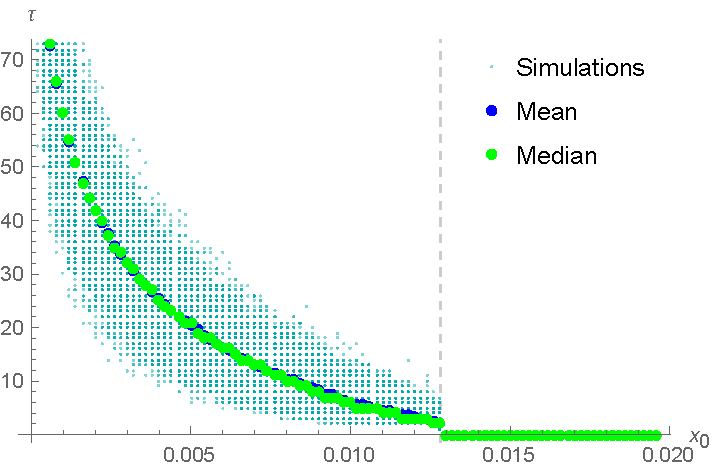
\includegraphics[width=\linewidth]{StopTime/1_BMtau.pdf}
		\end{minipage}
		& \begin{minipage}{.4\textwidth}
			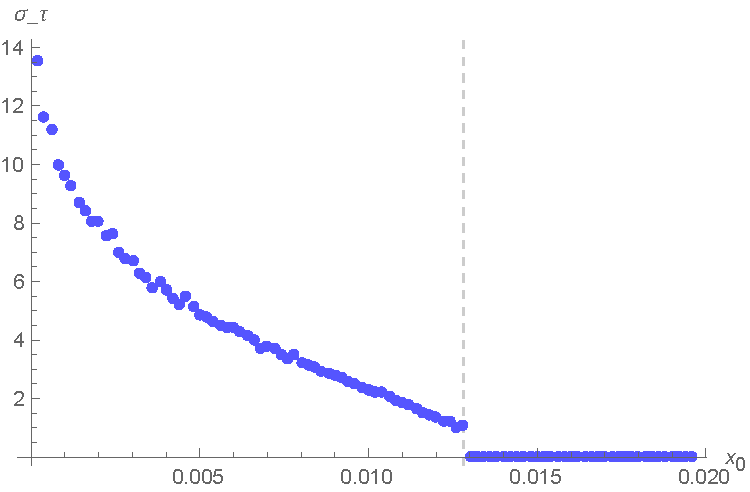
\includegraphics[width=\linewidth]{StopTime/1_BMsd.pdf}
		\end{minipage} 
	\\ \cline{2-4} 
		& CO & 
		\begin{minipage}{.4\textwidth}
			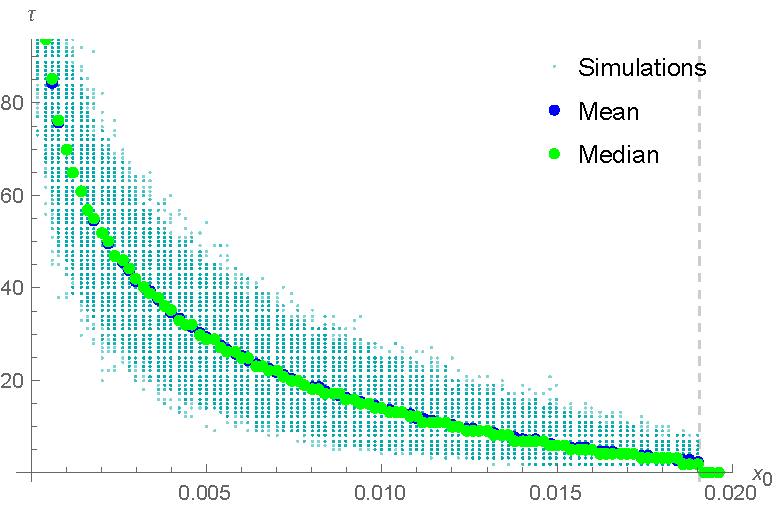
\includegraphics[width=\linewidth]{StopTime/1_COMtau.pdf}
		\end{minipage}
		& \begin{minipage}{.4\textwidth}
			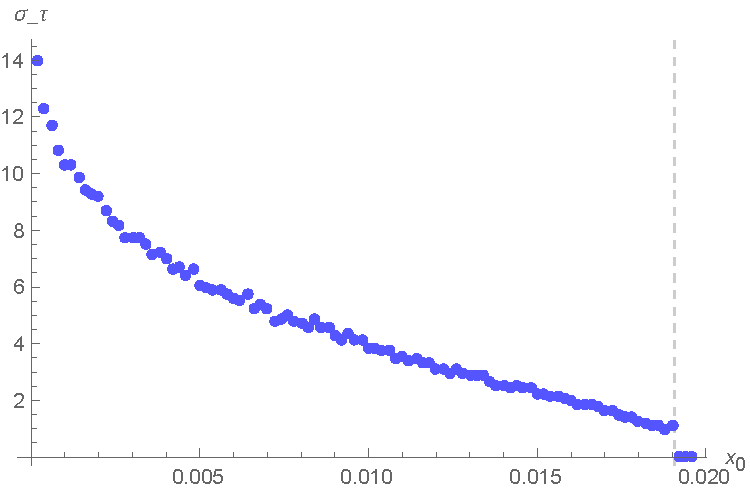
\includegraphics[width=\linewidth]{StopTime/1_COMsd.pdf}
		\end{minipage} 
	 \\ \hline
		\multirow{11}{*}{ \ref{chapter:2}} & B & 
			\begin{minipage}{.4\textwidth}
			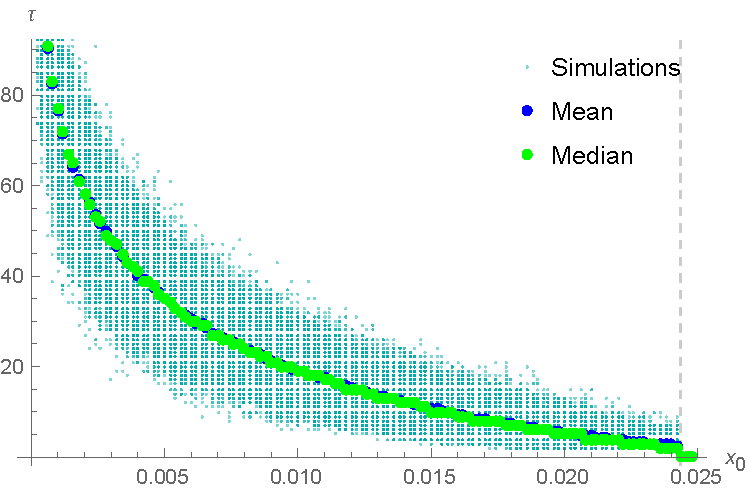
\includegraphics[width=\linewidth]
			{StopTime/2_BMtau.pdf}
		\end{minipage}
		& \begin{minipage}{.4\textwidth}
			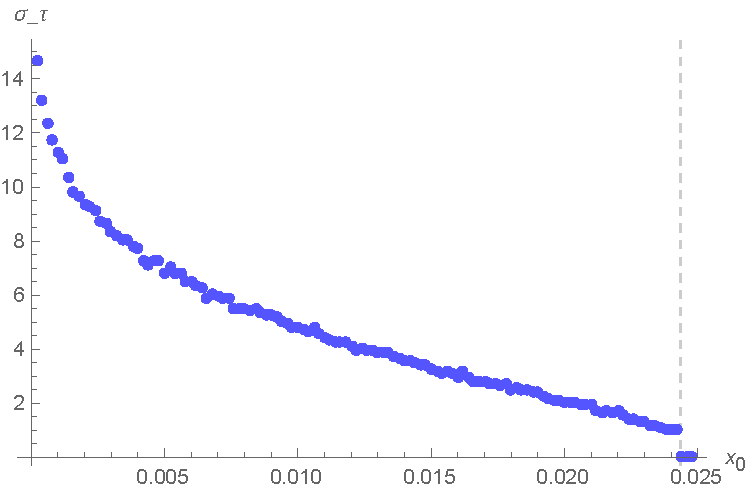
\includegraphics[width=\linewidth]
			{StopTime/2_BMsd.pdf}
		\end{minipage} 
	 \\ \cline{2-4} 
		& CO &
			\begin{minipage}{.4\textwidth}
			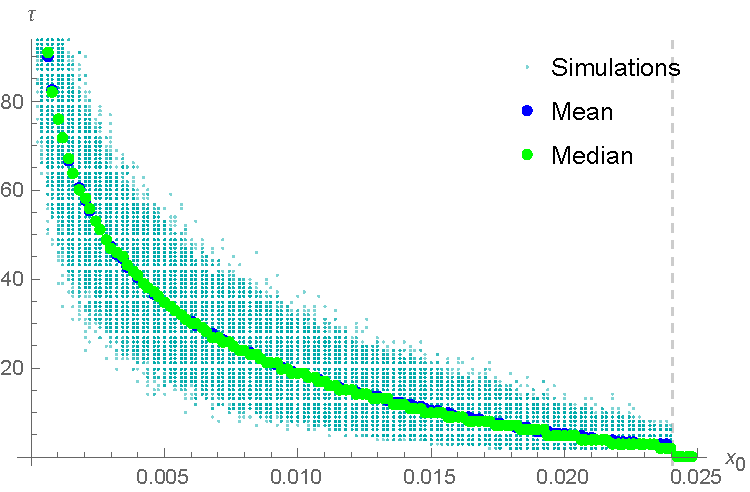
\includegraphics[width=\linewidth]
			{StopTime/2_COMtau.pdf}
		\end{minipage}
		& \begin{minipage}{.4\textwidth}
			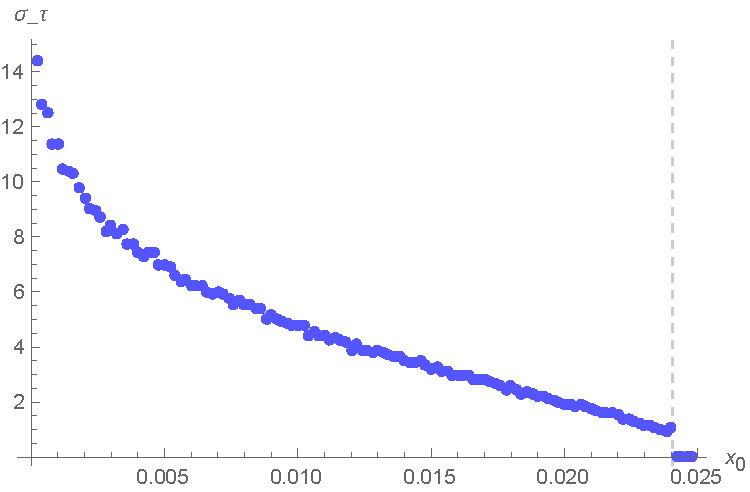
\includegraphics[width=\linewidth]
			{StopTime/2_COMsd.pdf}
		\end{minipage}   
	 \\ \hline
		\ref{chapter:3} & - &
		\begin{minipage}{.4\textwidth}
			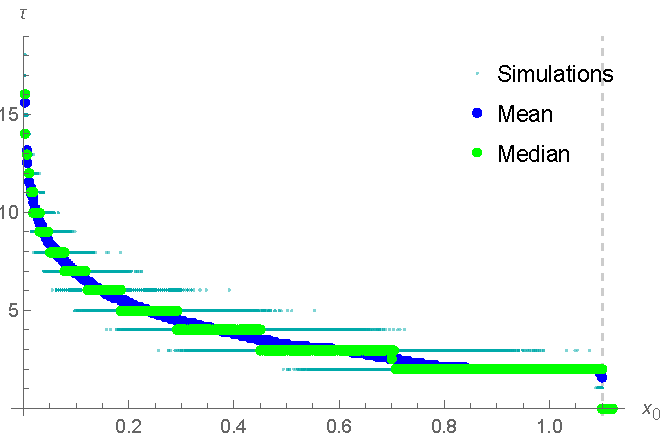
\includegraphics[width=\linewidth]
			{StopTime/3_BMtau1.pdf}
		\end{minipage}
		& \begin{minipage}{.4\textwidth}
			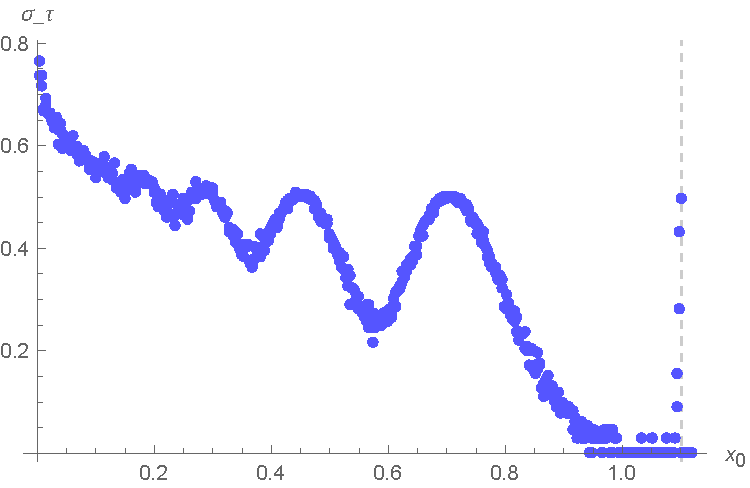
\includegraphics[width=\linewidth]
			{StopTime/3_BMsd.pdf}
		\end{minipage}    
	\end{tabular}
\label{tab1}
\end{table}
%\pagebreak
%\begin{figure}[!htb]
%	\begin{subfigmatrix}{6}
%		\subfigure[Mean \& Median of $\tau_B^*$ with respect to. \eqref{eq:sistema} ]{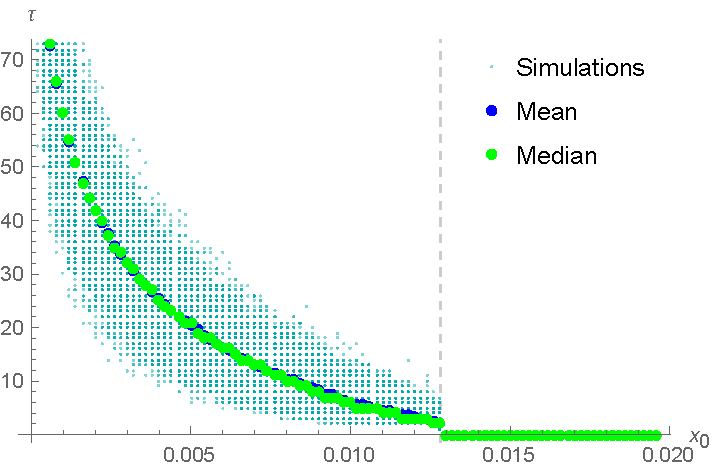
\includegraphics[width=0.35\textwidth]{StopTime/1_BMtau.pdf}}
%		\subfigure[Standard Deviation of $\tau_B^*$ with respect to. \eqref{eq:sistema} ]{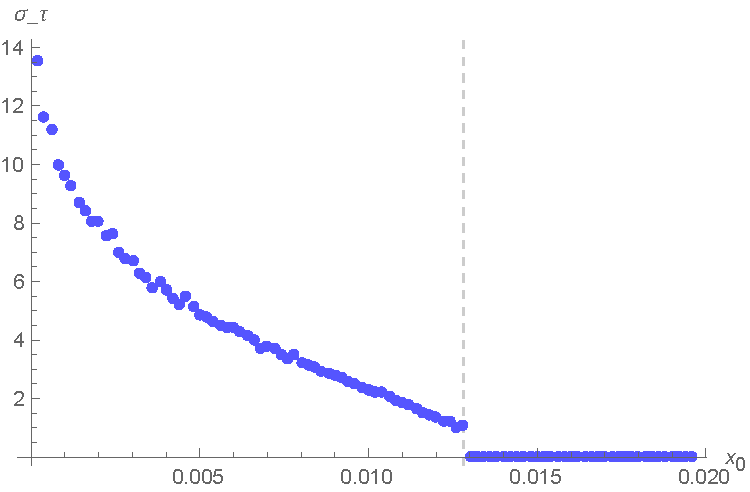
\includegraphics[width=0.35\textwidth]{StopTime/1_BMsd.pdf}}
%		\subfigure[Mean \& Median of $\tau_C^*$ with respect to. \eqref{eq:prob1_xC}]{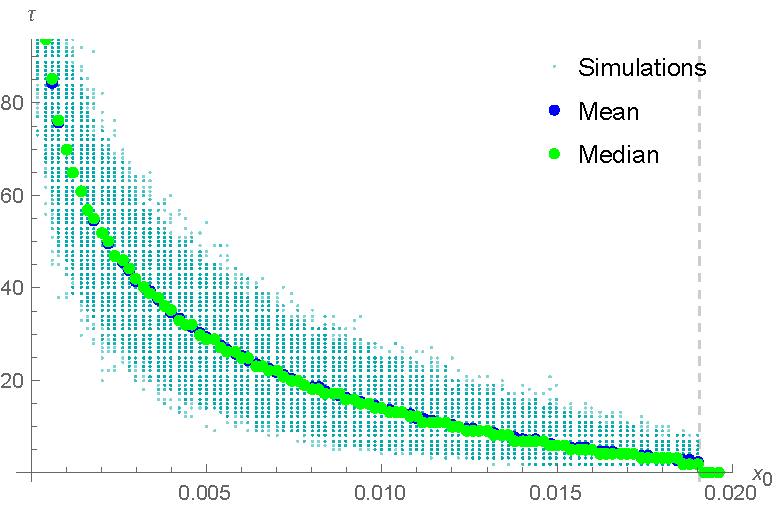
\includegraphics[width=0.35\textwidth]{StopTime/1_COMtau.pdf}}
%		\subfigure[Standard Deviation of $\tau_C^*$ with respect to. \eqref{eq:prob1_xC}]{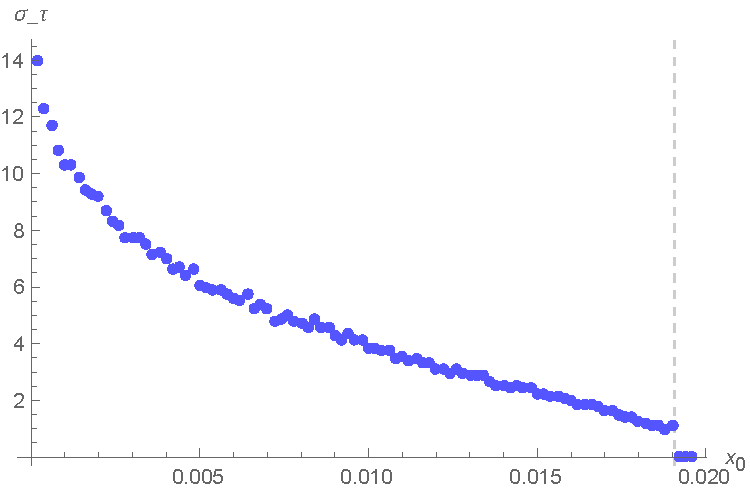
\includegraphics[width=0.35\textwidth]{StopTime/1_COMsd.pdf}}
%		\subfigure[Mean \& Median of $\tau_B^*$ with respect to. \eqref{2_xB} ]{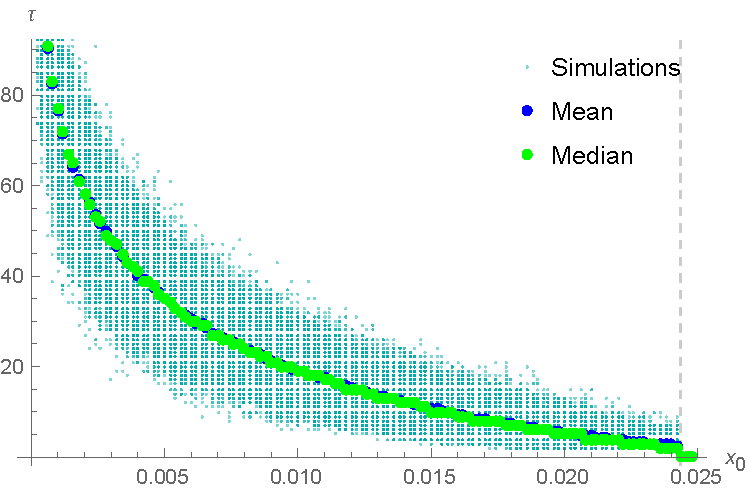
\includegraphics[width=0.35\textwidth]{StopTime/2_BMtau.pdf}}
%		\subfigure[Standard Deviation of $\tau_B^*$ with respect to. \eqref{2_xB} ]{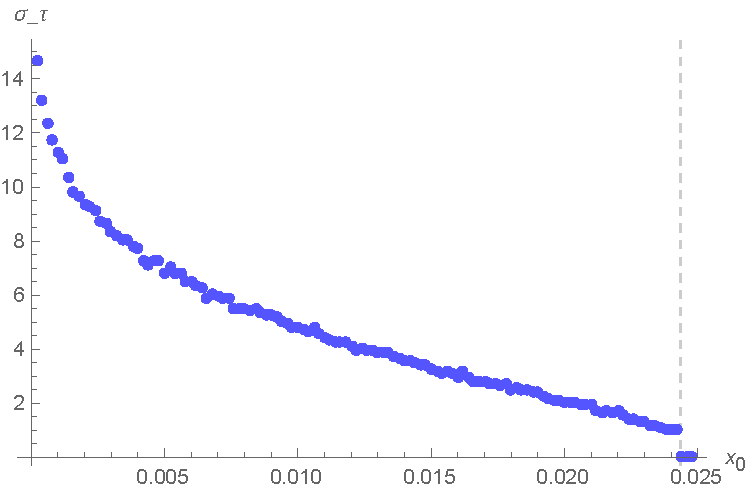
\includegraphics[width=0.35\textwidth]{StopTime/2_BMsd.pdf}}
%		\subfigure[Mean \& Median of $\tau_C^*$ with respect to. \eqref{eq:prob2_xC} ]{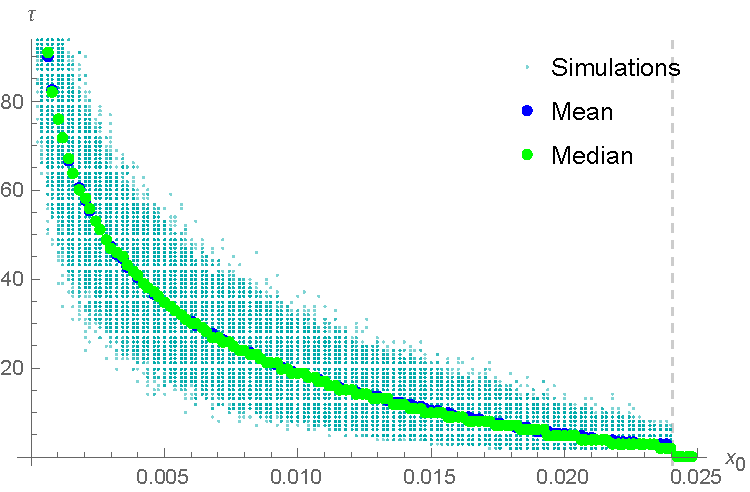
\includegraphics[width=0.35\textwidth]{StopTime/2_COMtau.pdf}}
%		\subfigure[Standard Deviation of $\tau_C^*$ with respect to. \eqref{eq:prob2_xC} ]{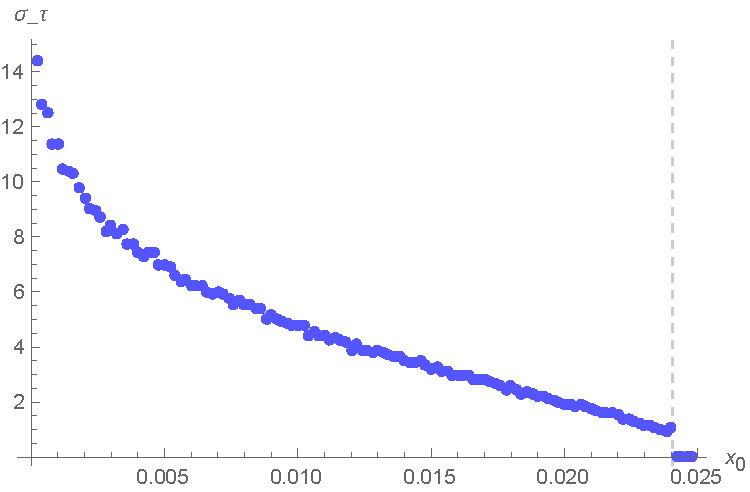
\includegraphics[width=0.35\textwidth]{StopTime/2_COMsd.pdf}}
%		\subfigure[Mean \& Median of $\tau_{1,A}^*$ with respect to. \eqref{eq:3_x1A}]{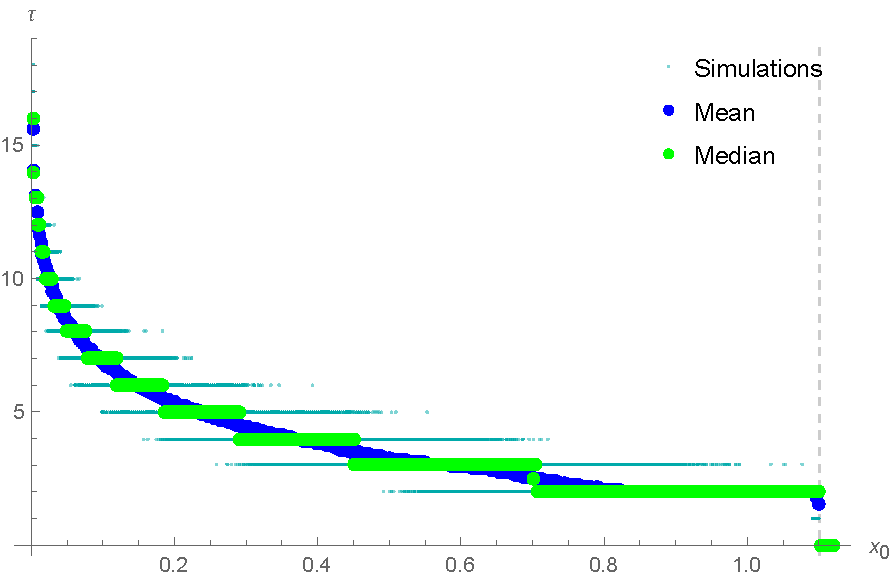
\includegraphics[width=0.35\textwidth]{StopTime/3_BMtau.pdf}}
%		\subfigure[Standard Deviation of $\tau_{1,A}^*$ with respect to. \eqref{eq:3_x1A} ]{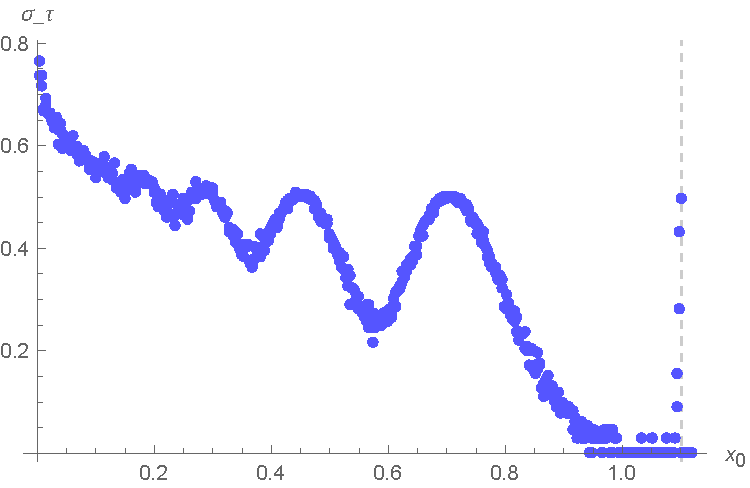
\includegraphics[width=0.35\textwidth]{StopTime/3_BMsd.pdf}}
%	\end{subfigmatrix}
%	\caption{Sensibility analysis of estimated mean and median (leftmost column) and standard deviation (rigthmost column) of the optimal investment time for each of the three situations studied, regarding different initial values $x_0$.}
%	\label{fig:stoptime_1}
%\end{figure}
%\pagebreak
%For all the analysis performed, we consider the same set of parameters used on respective Comparative Statics sections. The only exception stands for volatility, which we increase to $\sigma=0.1$, in order to obtain results within a larger variability.


%Despite $\sigma$, these are the same values used on Chapter \ref{chapter:3}. Note that by choosing $\eta=0.007$, we have that $\eta< \eta^*$ and thus we are in the situation where the firm has two decisions to make: when it should invest and start the simultaneous production; when it should stop  the simultaneous production and produce solely the new product.
%On Figure \ref{fig:stoptime_1} we can find the results obtained.

%Results are presented on Figure \eqref{fig:stoptime_1}.
On Table \ref{tab1}
%Figure \eqref{fig:stoptime_1}
the obtained results are presented, from which we conclude:
\begin{enumerate}
%	\item
%	Whenever a firm is interested to invest in a market on which the observed demand is greater than the demand that triggers the investment, it should immediately invest - obtaining a null expected waiting time with null variation;
%	\\ \textcolor{red}{Devo cortar esta conclusão?}
	\item The smaller the initial demand $x_0$, the longer the firm needs to wait to invest;
	\item The larger the demand value that triggers the investment, the longer the firm needs to wait to be advantageous to invest;
	\item The mean and the median of investment times are approximately equal, suggesting that the distribution of investment times is approximately symmetric;
	\item Both mean and median are of the same order of magnitude as the standard deviation. This suggests a high variability of the results obtained. Increasing the amount of sample paths simulated we observe no significant decrease of the variability, only a considerable longer computational running time.
\end{enumerate}
%Note that on every plot, the demand level that triggers the investment it is represented by a dashed line.

% As expected, for any initial value higher than the threshold,
%the firm is not expected to wait to decide - not only the mean and median are null, so it is the standard deviation.


%Observe that the smaller the initial value $x_0$, the higher (all) its respective measures are. 

%Also, the higher threshold level, the longer (in average and median) the firm will need to wait until it should invest. This situation is particularly noticeable on results regarding Chapter \ref{chapter:1}.


We suspect that the noticeable logarithmic behaviour of simulated optimal times' mean comes from the fact that
\begin{align*}
\mathds{E}^{X_0}[X_\tau]=X_0 e^{\mu \tau} \ \Leftrightarrow \ \tau= \frac{1}{\mu} \log \left|  \frac{\mathds{E}^{X_0}[X_\tau]}{X_0} \right|
\end{align*}

Considering the estimate of the optimal investment time given by the sample mean of the simulated exercising times (with respect to each initial value tested; here denoted by $\hat{\tau}$) and noticing that $X_\tau$, written above, corresponds to a threshold (with respect to a particular investment situation; here denoted by $x^*$), it follows that
\begin{align}
 \hat{\tau}=\frac{1}{\mu} \log \left|  \frac{x^*}{X_0} \right|, \quad \text{considering} \ x^*> X_0.
\end{align}

%$\hat{\tau}$ is taken as the sample mean. %he the estimator of the mean is consider to b
The case $x^*\leq X_0$ is not here addressed since it immediately implies that the firm invests right away, resulting in a null expected waiting time.
%The results concerning the mean and the median of the optimal investment times have an intuitive explanation: when starting with a small demand level (or considering an higher threshold), one expects to wait more time until the demand level reaches the threshold demand level, than when starting with an higher level (or with a smaller threshold). However the result concerning the standard deviation is not that obvious. It can arise due to the randomness of the GBM and its time increasing variance, respectively given by $Var(X_t)=X_0^2 e^{2\mu t}(e^{\sigma^2 t} -1), \ \forall t\geq0, \mu \geq 0$, which allows the sample path to be more diverse (either in observed states as in running lenght) and thus obtain also more distinct stopping times.
%Also, observe that for higher threshold levels, in average and median, the firm will need to wait more time until it is able to invest. This fact is particularly noticeable on the first two rows, whose results are taken with respect to the first situation (Section \ref{chapter:1}).




%We highlight here, as well, the fact that the mean and the median of investment times is approximately equal, suggesting that the distribution of investment times is approximately symmetric.

On the last row we find the results concerning the optimal time to invest in a new product and start to produce, simultaneously, the old and new products, as studied on Chapter \ref{chapter:3}.
The noticeable \textit{step} behaviour of both simulated values and respective mean is a consequence of the unitary time step considered during the simulation and the scale of the results obtained. Note that this implies a more irregular standard deviation as presented on the last row of Table \ref{tab1}.
Although this behaviour is not easily detectable on the other situations, since the results obtained are in a larger scale, one expects that they behave the same way.
%Although its simulations and median are presented in a (clear) step format, they have a similar behaviour has 
% to have a median more be sparser (regarding the median) and more oscillated (regarding the standard deviation) than the others, they have a similar behaviour to the previous ones showed. Changes are only more noticeable due to the range of values obtained and the respective ratio between them and \texttt{xStep}.


Taking now into account the optimal time to stop the production of the established product, studied on Chapter \ref{chapter:3}, we obtain the results presented on Table \ref{stoptime_t}.
\begin{table}[!htb]
	\caption{Sensitivity analysis of estimated mean, median and standard deviation of optimal time to decide stop the production of the established product when considering an observed demand $x_{1,A}^*$.}
	\centering
	\vspace{2mm}
	\begin{tabular}{ccc}
		Mean & Median & Standard Deviation \\ \hline
		5.49 & 5.00 & 0.77
	\end{tabular}
\label{stoptime_t}
\end{table}

Recall that we consider the demand process to start at $x_{1,A}^*$, since this is the demand level observed at the instant the firm invests on the innovative product. Therefore, mean and median are taken considering as \textit{initial instant} the time at which the firm decides to invest in the new product and start the simultaneous production, that is, $\tau^*_{1,A}=\inf \{ t\geq 0: X_t \geq x^*_{1,A} \}$. Thus, the mean/median presented should be read as the mean/median time after the investment on the new product was done. To obtain the estimated mean/median time for which the firm produces solely the new product, one should add the value presented on Table \ref{stoptime_t} to the one obtained as the mean/median time to invest in the new product, for a given initial demand value $x_0$.    

We note that, in this case, it seems that the results do not have large volatility, and thus we may suggest that the sample mean and median are good descriptors of the optimal time it takes to decide to stop the old product's production.



%\pagebreak
\section{Sensitivity of the optimal investment times with respect to volatility, $\sigma$}

In this section we are interested to observe how optimal investment times behave with market's uncertainty.

\subsubsection{Methodology}

We analyse all models concerning the three previous chapters, by studying the respective investment times concerning changes on demand's volatility, which is consider to vary between 0.01 and 0.5. By considering two different initial demand values ($x_0=0.001$ and $x_0=0.01$), we study its behaviour by analysing its absolute and relative variation, following the procedure described on the undermentioned diagram.

\vspace{0.5cm}
\begin{tikzpicture}[
level 1/.style={sibling distance=10cm},
edge from parent/.style={->,draw},
>=latex]

% root of the the initial tree, level 1

\node[root] (r) {\textbf{1.} Fix parameters of interest:
};

\node[level 3, below of = r, yshift=-2cm] (p) {
	$\bullet$ $\sigma$Min=0.01\\
	$\bullet$ $\sigma$Max=0.5\\
	$\bullet$ timeStep=1\\
	$\bullet$ horizon=1500\\
	$\bullet$ Nsamplepaths=500\\
	$\bullet$ xthreshold: the ones associated to each chapter
};

\node [root, below of = p, yshift=-4.5cm] (treino) { \textbf{2.}  Simulate Nsamplepaths=500 demand processes using \texttt{estTau} function\\ \underline{Output:} collection of values $(\sigma_j, \bar{\tau}_j)$ with $\bar{\tau}_j$ representing the mean of the investment times concerning the 500 sample paths simulated w.r.t. $\sigma_j$};

%\node [root, below of = treino, yshift=-2cm] (val) {\textbf{3.}  For each $x_{0j}$,\\
%	calculate mean, median and standard deviation of observed optimal investment times $\tau_{j}$ using obtained values $\{\tau_{ji} \}_{i \in \{ 1,...,1000\} }$};

\node [root, below of = treino,  xshift=-4cm, yshift=-3cm] (plot1) {\textbf{Plot 1}:\\ estimated expected optimal investment times w.r.t. $\sigma$
	\begin{flushleft}
	$\bullet$ $x_0$=0.001: \textit{lighter colours}\\
	$\bullet$ $x_0$=0.001: \textit{darker colours}\\
	\end{flushleft}
};

\node [root, below of = treino,  xshift=4cm, yshift=-3.3cm] (plot2) {\textbf{Plot 2}:\\ variation rate of estimated expected optimal investment times w.r.t. $\sigma$ calculated accordingly to
\eqref{var}
\begin{flushleft}
$\bullet$ $x_0$=0.001: \textit{lighter colours}\\
$\bullet$ $x_0$=0.001: \textit{darker colours}\\
\end{flushleft}
};


% lines from each level 1 node to every one of its "children"


\draw[->] (r) -- (p);
\draw[->] (p) -- (treino);

\draw[->] (treino) -- (plot1);
\draw[->] (treino) -- (plot2);
\end{tikzpicture}

The absolute variation is (straightforward) given by the mean of simulated optimal investment times with respect to each value of $\sigma$.

The relative variation is analysed accordingly to the variation rate (here denoted by $\triangle_n \% $), which is calculated as
\begin{equation}
\triangle_n \% = \frac{f(\sigma_n)-f(\sigma_{n-1})}{\sigma_n-\sigma_{n-1}} \times 100 \% \  \ \text{with} \ \ \sigma_n=0.01+n\times0.01, \ \ n=\left\lbrace 0,..., \frac{\sigma Max}{\sigma Step}=50 \right\rbrace,
\label{var}
\end{equation}
where $f$ corresponds to the sample mean of optimal times simulated w.r.t. a certain volatility.

Since it's not deterministic that all sample paths reach the demand threshold, we define a time horizon to assure that the algorithm runs in \textit{human-time} and that it ends. On the results showed hereunder a \texttt{horizon} of 1500 time units\footnote{This value is used as input in \texttt{stopTimemod} function, which is an auxiliary function of \texttt{estTau}. For further details check Appendix \ref{chapter:appendixVectors}.} is considered. As before we consider a time step of one time unit.

Once again the analysis regarding the optimal time to abandon the simultaneous production, referred on Chapter \ref{chapter:3} and denoted by $\tau_2$, consider as initial demand value $x_1,A$ (that is the demand level observed when the firm invests in the innovative product). Also, the values presented regarding $\tau_2$ sould be read as: \textit{after the investment on the innovative product, the firm is expected to wait $\tau_2$ time units to abandon the production of the old product.}




%
%As done before, we consider the same values fixed in previous comparative sections, namely on Chapter \ref{chapter:3}.
%
%Considering a model and respective parameters fixed, \texttt{stopTimemod} simulates \texttt{NsamplePaths}=500 demand sample paths, recording the instant at each of them either reaches the demand threshold considered or reaches time \texttt{horizon}. Since it's not deterministic that all sample paths will reach the threshold, this last condition is crucial to assure that the algorithm runs in \textit{human-time}. On the results showed hereunder we consider \texttt{horizon}=1500 time units.
%
%Function \texttt{estTau} calculates the mean of the investment times obtained by \texttt{stopTimemod} per each volatility level $\sigma_i$, which starts in 0.01 and it is incremented $i$-th times 0.01, until reaches \texttt{$\sigma$ Max}=0.5, that is $\sigma_i=0.01+i \times 0.01 \in [0.01,0.5]$.
%
%We run \texttt{estTau} for each of the models studied - either benchmark or capacity optimization model - and considering two initial points $x_0 \in \{0.001, \ 0.01 \}$. We also evaluate as well the respective threshold values and optimal capacity in order to compare results obtained, based on their absolute value and variation.
%
%In order to calculate the variation, we consider a partition of (0,0.5] with $0.5/0.01=50$ subintervals of the form $I_n=(\sigma_n, \sigma_{n-1}],\ n \in \{2,...,50\}$. Denoting the percentage of variation associated to the $I_n$ interval by $\triangle_n \%$, it follows that for $n \in \{2,...,50\}$ it is given by
%$$\triangle_n \% = \frac{f(\sigma_n)-f(\sigma_{n-1})}{\sigma_n-\sigma_{n-1}} \times 100 \%,$$
%with $f$ being any of the measures of interest - mean of investment times, demand threshold or optimal capacity -, which only depends on the volatility considered.
%
%


\subsubsection{Results}

The numerical results for the investment times related to both models (the benchmark and the optimal capacity models) as a function of $\sigma$ (the volatility of the demand) obtained are presented on Table \ref{res2}. 

For the sake of completeness, we include also the corresponding investment thresholds and the optimal capacity level. These are not obtained by simulation. They are rather the implementation of equations presented on the previous respective chapters.
However, due to the contrasting order of magnitude of the optimal investment times with the optimal capacity $K^*$ and demand thresholds, the last ones are only considered for the analysis of the relative variation, on the rightmost column.

\begin{table}[!htb]
	\caption{Sensitivity analysis of the (estimated) mean of optimal investment time w.r.t. the demand's volatility, regarding different initial values $x_0 \in \{0.001, \ 0.01\}$.}
	\begin{tabular}{c|c|c}
		\hline
		Chapter & Absolute variation & Relative variation \\ \hline
		\ref{chapter:1} & \begin{minipage}{.45\textwidth}
			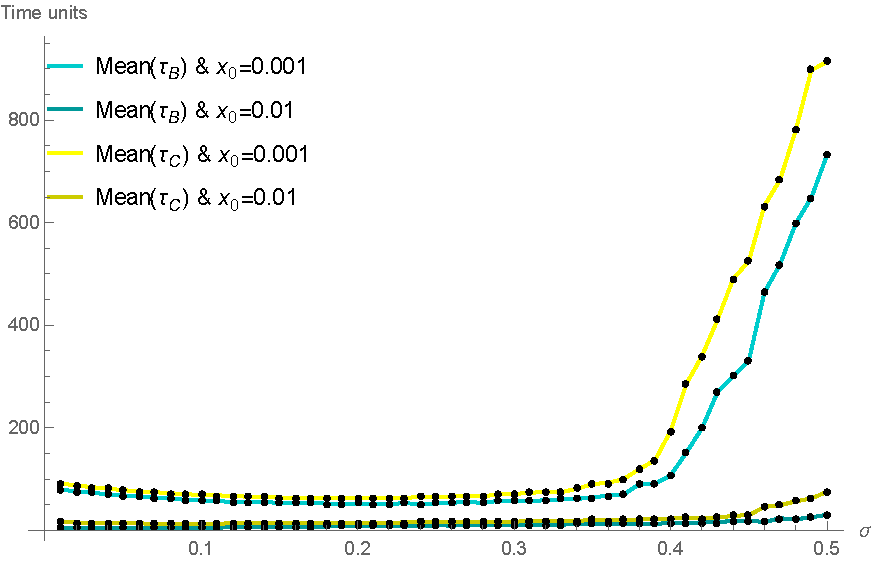
\includegraphics[width=\linewidth]{StopTime/1_meantauSP500H1500.pdf}
		\end{minipage}
	 & \begin{minipage}{.45\textwidth}
	 	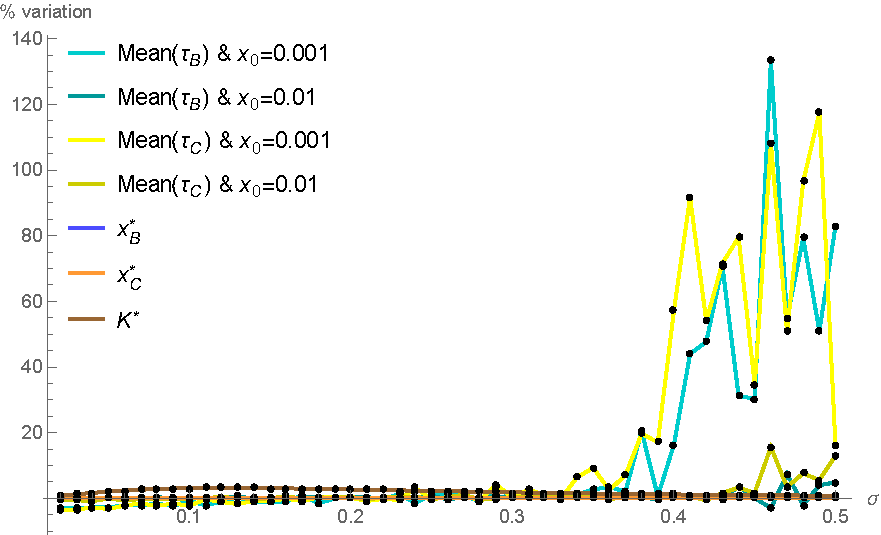
\includegraphics[width=\linewidth]{StopTime/1_var1.pdf}
	 \end{minipage}
  \\ \hline
		\ref{chapter:2} & 
		\begin{minipage}{.45\textwidth}
			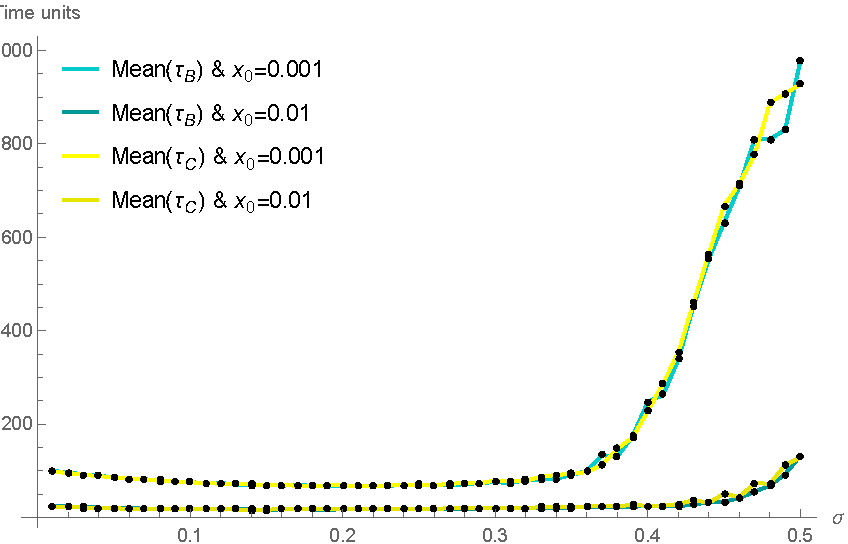
\includegraphics[width=\linewidth]{StopTime/2_meantau1.pdf}
		\end{minipage}
		& \begin{minipage}{.45\textwidth}
			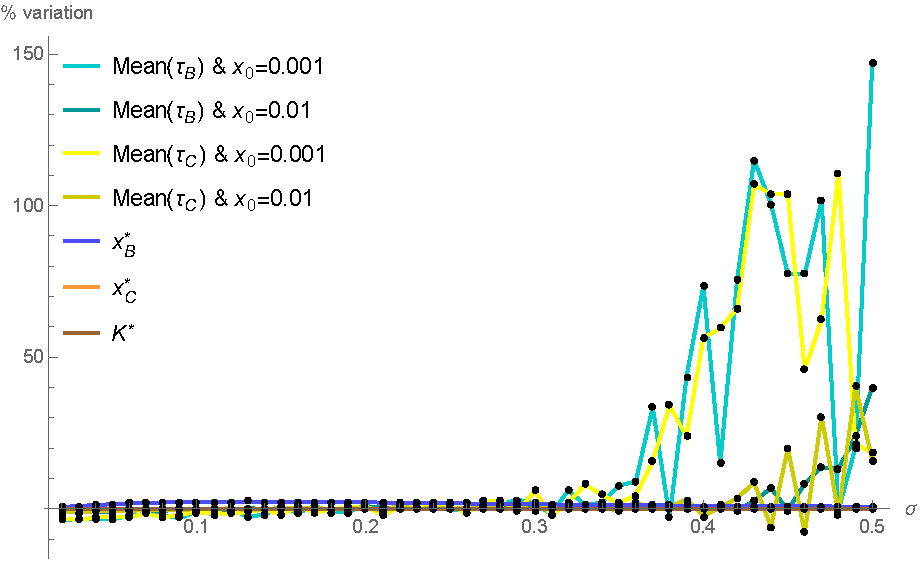
\includegraphics[width=\linewidth]{StopTime/2_varSP500H1500.pdf}
		\end{minipage}
		 \\ \hline
		\ref{chapter:3} & \begin{minipage}{.45\textwidth}
			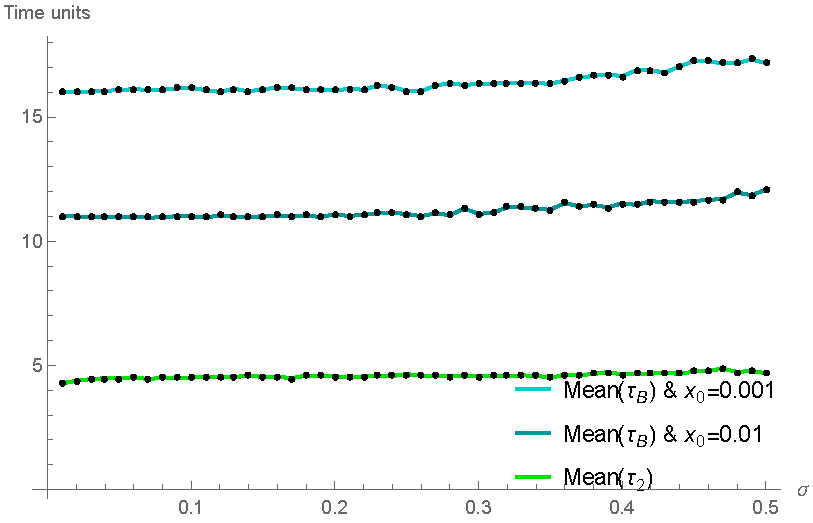
\includegraphics[width=\linewidth]{StopTime/3_meantau1.pdf}
		\end{minipage}
		& \begin{minipage}{.45\textwidth}
			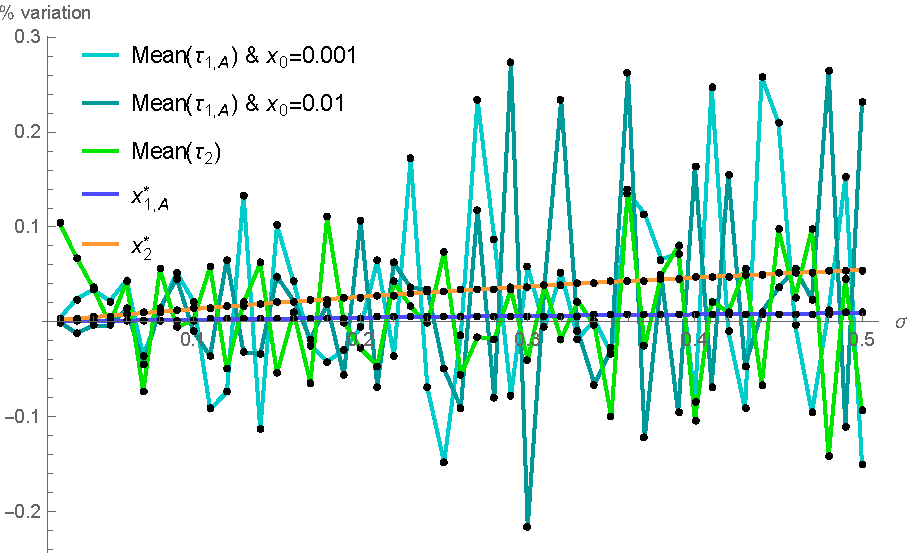
\includegraphics[width=\linewidth]{StopTime/3_var1.pdf}
		\end{minipage} \\ \hline
	\end{tabular}
\label{res2}
\end{table}


Confronting the results of performed simulations, regarding both models on chapters \ref{chapter:1} and \ref{chapter:2}, above presented with the numerical results present on Appendix \ref{chapter:appendixVectors}, the following conclusions are pointed:
\begin{enumerate}
	
	
	
	\item The mean time to undertake the decision is stable for a significant range of values $\sigma$ (i.e., the mean seems not to change significantly for values $\sigma \leq 0.35$). But then it shows a considerable increasing trend, more pronounced on the optimal capacity model;
	
	\item  The observed mean of the investment times has a non-monotonic behaviour:
	 \begin{itemize}
	 	\item For small values of $\sigma$ (approximately smaller than 0.2),  as slight decreasing tendency, which leads to anticipate the investment decision, is observed as the volatility increases. This is not an expected result from real option approach - for which an increasing volatility leads to a late decision \cite{dixit:book} -, however it might be justifiable by the crossed-effect of a small rate growing of the thresholds for small values of $\sigma$ (as seen on Figure \ref{fig:sigm} (b) and Figure \ref{fig:2_x2} (b)) and the impact of a small volatility level on the demand process; 
	 	\item For large values of $\sigma$ (approximately greater than 0.2), we observe that a larger uncertainty on the market seems to likely postpone the investment decision;
	 \end{itemize}

	\item There seems to exist no relation between the behaviour of the mean time to undertake the decision and the demand threshold level or the optimal capacity associated.	
\end{enumerate}



%The results regarding the behaviour of the investment times 
For the case when the firm is already in the market and may either replace or add a new product (Chapter \ref{chapter:3}), the investment times (presented on the last row), have a different behaviour from the previous ones. We note that for this case the expected times (both for the investment and for the replacement time) are more stable that in the other two cases, in the sense that changes on $\sigma$ do not affect them as significantly as in the previous cases. We do not have any explanation for this fact. However we do suspect that it is related with the fact that quite different values are considered for the numerical simulation of the chapter \ref{chapter:3} than for chapters \ref{chapter:1} and \ref{chapter:2}.  


\section{Sensitivity of the optimal investment times with respect to the crossed-effect between initial demand value, $x_0$, and volatility, $\sigma$}

Additionally we study the crossed-effect of both initial demand value and volatility. This is achieved by analysing the frequency of the optimal investment times obtained through their histogram representation.

\subsubsection{Methodology}

Per each set of values chosen, we simulate 500 demand sample paths, using function \texttt{hist}\footnote{For further details, check Appendix \ref{chapter:appendixVectors}.}, until they reach either the respective demand threshold or the time horizon, here set as 1500 time units.
The set of parameters considered was the same as in the respective comparative statics sections.

As previously noticed, since the results obtained for chapters \ref{chapter:1} and \ref{chapter:2} and both benchmark and capacity optimization models are quite similar, we only represent in this thesis here the results regarding chapters \ref{chapter:1} and \ref{chapter:3}.


\subsubsection{Results}

Table \ref{hist} shows the results regarding the benchmark model associated to the situation on which a firm is not active in the market and wants to enter it with an innovative product, deduced on Chapter \ref{chapter:1}. The results obtained can be extended to the optimal investment time deduced on Chapter \ref{chapter:2}.

\begin{table}[!htb]
	\caption{Histograms of simulated optimal investment times of the benchmark model w.r.t. the situation for which a firm is not active in the market and wants to enter it with a new product (Chapter \ref{chapter:1}), considering initial demand values $x_0=\{0.001,\ 0.01\}$ and demand's volatilities $\sigma=\{0.001, \ 0.1, \ 0.5 \}$.}
	\begin{tabular}{c|c|c}
		\hline
		Volatility & $x=0.001$ & $x=0.01$ \\ \hline
		$\sigma=0.001$ & \begin{minipage}{.45\textwidth}
			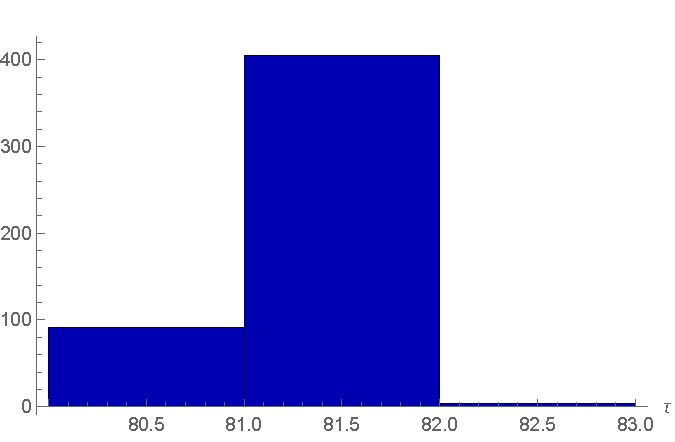
\includegraphics[width=\linewidth]{StopTime/x001o001.pdf}
		\end{minipage}
		& \begin{minipage}{.45\textwidth}
			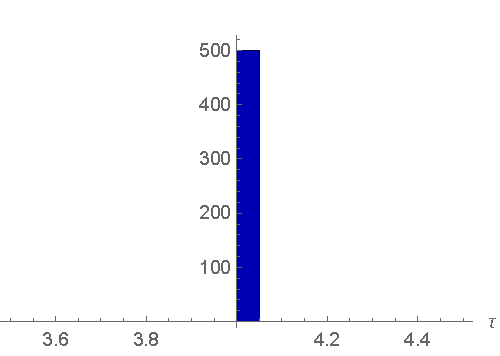
\includegraphics[width=\linewidth]{StopTime/x01o001.pdf}
		\end{minipage}
		\\ \hline
		$\sigma=0.1$ & 
		\begin{minipage}{.45\textwidth}
			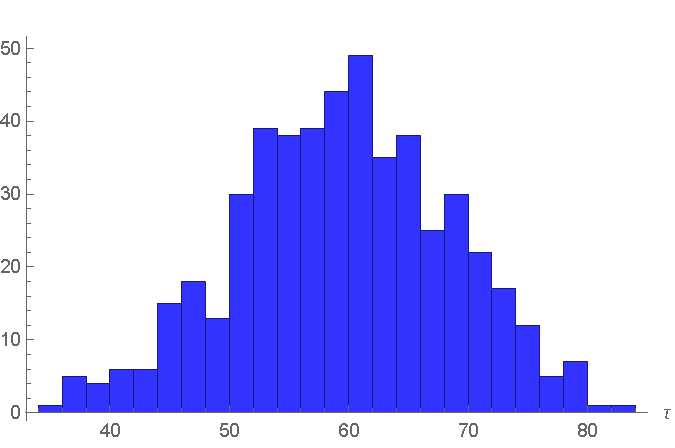
\includegraphics[width=\linewidth]{StopTime/x001o1.pdf}
		\end{minipage}
		& \begin{minipage}{.45\textwidth}
			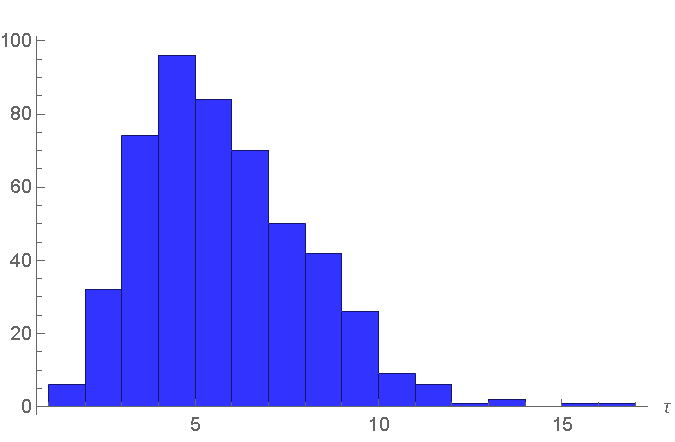
\includegraphics[width=\linewidth]{StopTime/x01o1.pdf}
		\end{minipage}
		\\ \hline
		$\sigma=0.5$ & \begin{minipage}{.45\textwidth}
			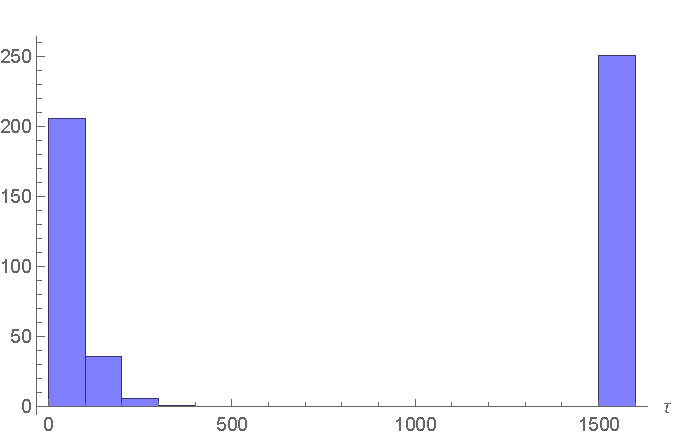
\includegraphics[width=\linewidth]{StopTime/x001o5.pdf}
		\end{minipage}
		& \begin{minipage}{.45\textwidth}
			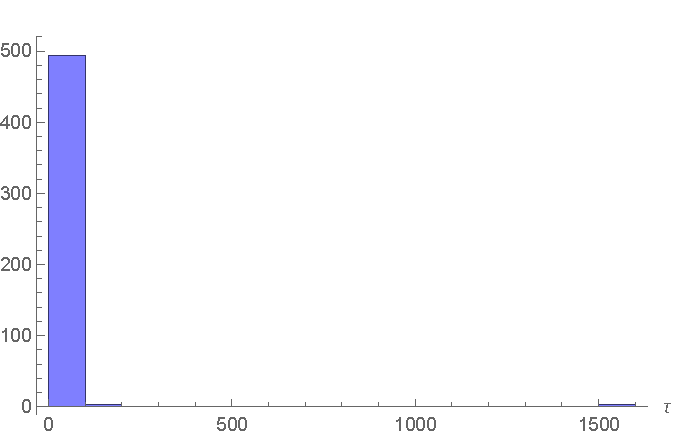
\includegraphics[width=\linewidth]{StopTime/x01o5.pdf}
		\end{minipage} \\ \hline
	\end{tabular}
	\label{hist}
\end{table}


We conclude the following aspects:
\begin{enumerate}
	\item The smaller the uncertainty in the market, the lower is the variability of the waiting time to invest.
	However, as previously concluded from Table \ref{res2}, this is not associated to the lowest waiting times.
	When considering $\sigma=0.001$ and $x_0=0.1$ we observe that for all the demand processes simulated, the firm enters the market after 4 time units. This is not a surprising, as we are choosing a really low value of volatility, leading to an almost deterministic process;
	
	\item The larger the volatility, the larger is the number of demand sample paths that do not reach the demand level that triggers the investment within the horizon defined (of 1500 time units). This result is in accordance to the significant growth of the waiting time when on markets with a large uncertainty, as observed on Table \ref{res2};
	
	\item A significant reduction on the waiting time until investment is observed when the initial demand value increases. This result is also noticeable in Table \ref{tab1}, on which the waiting time seems to have a logarithmic dependence on the initial value chosen;
	
	\item Assesing the normality of the optimal investment times,, recurring to a Shapiro-Wilk test \cite{sw}\footnote{On Mathematica it is given by \texttt{ShapiroWilkTest} function: \url{https://reference.wolfram.com/language/ref/ShapiroWilkTest.html}}
		, we obtain that solely for $x=0.001$ and $\sigma=0.1$, the normality is verified for the usual significance levels $(1\%, \ 5\%, \ 10\%, \ 15\%)$ - since we obtain a p-value $\simeq 0.264$.
\end{enumerate}


\vspace{3mm}
Now we analyse the situation on which a firm is already active, but wants to enter the market with an innovative product, allowing a simultaneous production period, as described on Chapter \ref{chapter:3}. Here we only analyse the threshold that triggers the introduction of the innovative product in the market, $x^*_{1,A}$, since it is dependent on the initial demand value (while the threshold that triggers the removal of the old product, $x_2$, it is not).


\begin{table}[!htb]
	\caption{Histograms of simulated optimal investment times w.r.t. the situation when an already active firm wants to introduce an innovative product in the market, allowing a simultaneous production period, considering initial demand values $x_0=\{0.001,\ 0.01\}$ and demand's volatilities $\sigma=\{0.001, \ 0.1, \ 0.5 \}$.}
	\begin{tabular}{c|c|c}
		\hline
		Volatility & $x=0.001$ & $x=0.01$ \\ \hline
		$\sigma=0.001$ & \begin{minipage}{.45\textwidth}
			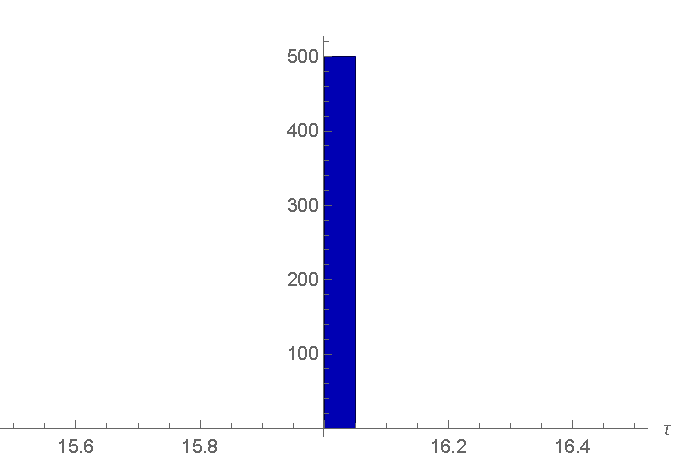
\includegraphics[width=\linewidth]{StopTime/3x001o001.pdf}
		\end{minipage}
		& \begin{minipage}{.45\textwidth}
			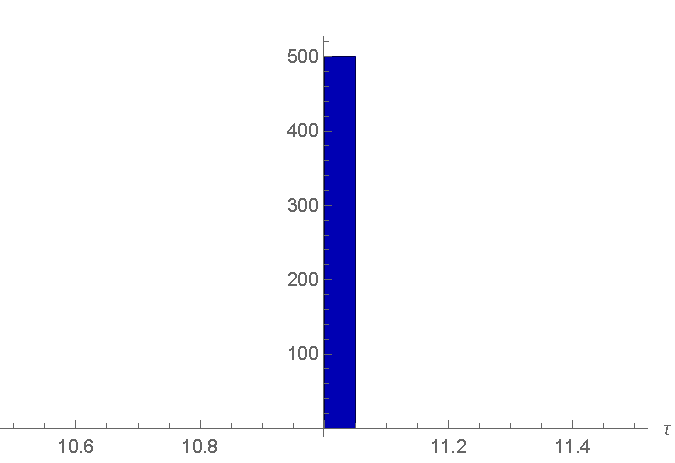
\includegraphics[width=\linewidth]{StopTime/3x01o001.pdf}
		\end{minipage}
		\\ \hline
		$\sigma=0.1$ & 
		\begin{minipage}{.45\textwidth}
			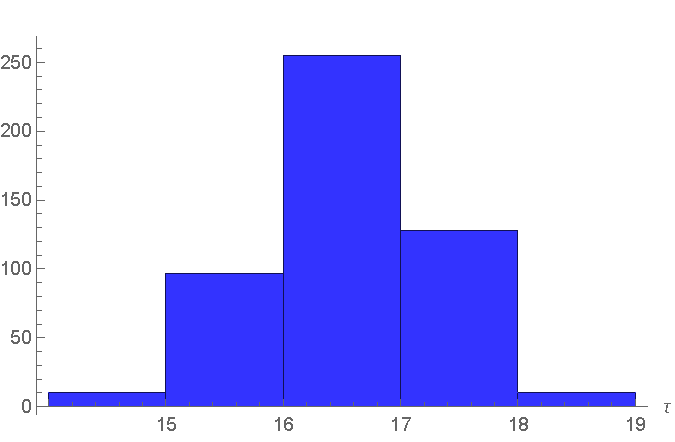
\includegraphics[width=\linewidth]{StopTime/3x001o1.pdf}
		\end{minipage}
		& \begin{minipage}{.45\textwidth}
			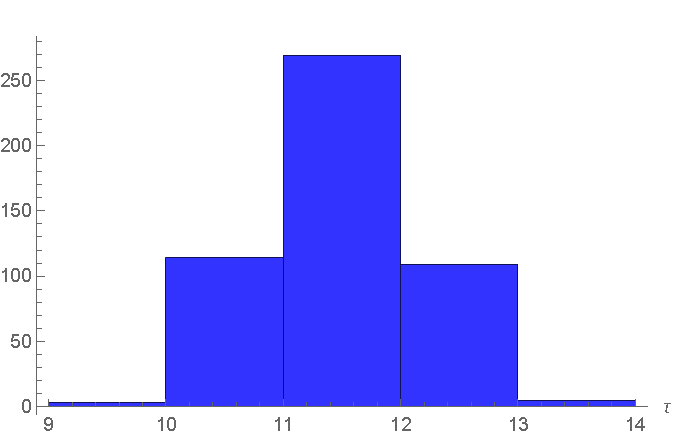
\includegraphics[width=\linewidth]{StopTime/3x01o1.pdf}
		\end{minipage}
		\\ \hline
		$\sigma=0.5$ & \begin{minipage}{.45\textwidth}
			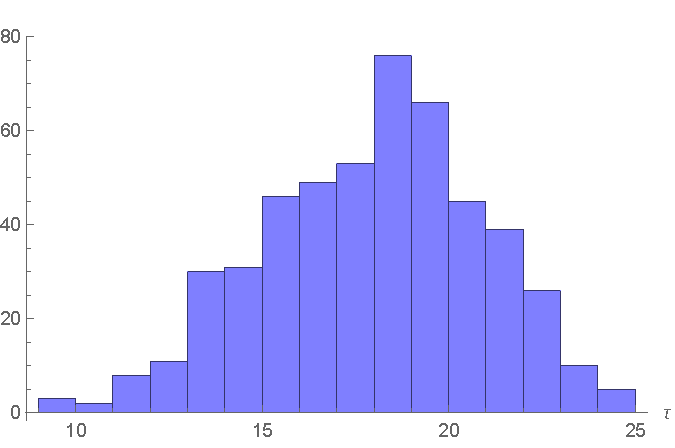
\includegraphics[width=\linewidth]{StopTime/3x001o5.pdf}
		\end{minipage}
		& \begin{minipage}{.45\textwidth}
			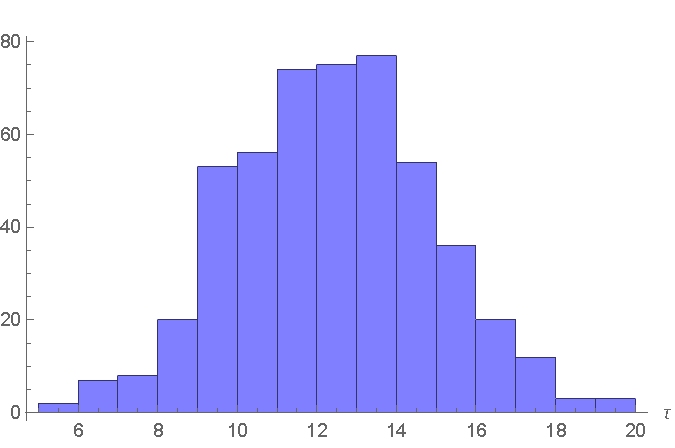
\includegraphics[width=\linewidth]{StopTime/3x01o5.pdf}
		\end{minipage} \\ \hline
	\end{tabular}
	\label{hist2}
\end{table}



From the results presented on Table \ref{hist2}, the following conclusions are taken:
\begin{enumerate}
	\item The larger the uncertainty in the market, the larger the variance observed on the simulated optimal investment times;
	
	\item There are no significant changes on the behaviour of the simulated optimal investment times with the initial value of the demand observed. Nevertheless, we observe that larger initial demand values reflect on smaller waiting times until it is advantageous for the firm to invest, as concluded from Table \ref{tab1};
	
	\item In none of the situations the time horizon defined (of 1500 time units) was reached. This is in accordance to the uniformity observed on Table \ref{res2};
	
	\item In none of the situations exists statistical evidence that the waiting times are normally distributed - the largest p-value obtained when performing Shapiro-Wilk test \cite{sw}: $4\times 10^{-5}$.
\end{enumerate}















%Despite the initial demand value and volatility, the set of parameters considered, regarding each model, was the same as chosen in the previous section. We consider here as well a \texttt{timeStep} of one time unit. For each of the three situations studied, we present the graphical result and a table in which are numerically presented the diverse measures analysed regarding volatility increments of 0.05.
%
%\vspace{3mm}
%$\bullet$ \textbf{Situation on Chapter \ref{chapter:1}: firm has no products in the market and wants to introduce a new one}
%
%On Figure \ref{fig:vol_1} we observe that both optimal investment times have a non-monotonic behaviour with the volatility. Even when the threshold level and the optimal capacity level increase with it.
%
%One can also note that the optimal investment times for both benchmark and capacity optimization models increase significantly for volatilities $\sigma>0.35$. This effect is more significant when considering a smaller initial value $x_0$.
%
%
%
%
%
%
%
%\begin{figure}[!ht]
%	\begin{subfigmatrix}{3}
%		\subfigure[(Estimated) mean of optimal investment times. ]{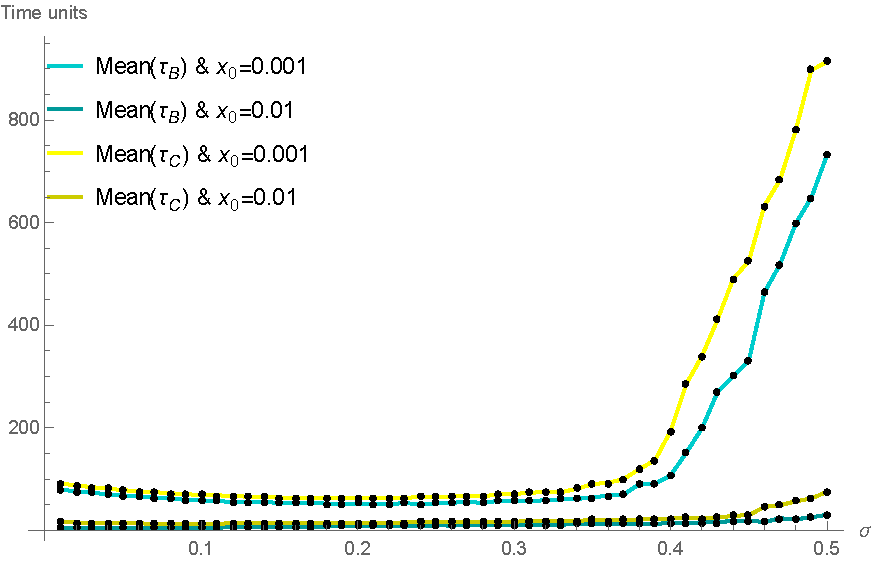
\includegraphics[width=0.32\textwidth]{StopTime/1_meantauSP500H1500.pdf}}
%		\subfigure[Demand threshold. ]{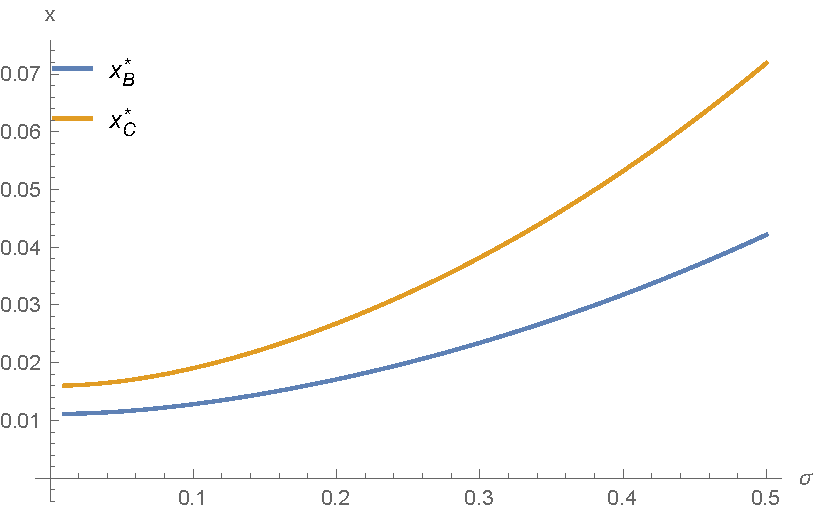
\includegraphics[width=0.32\textwidth]{StopTime/1_x.pdf}}
%		\subfigure[Optimal capacity level.]{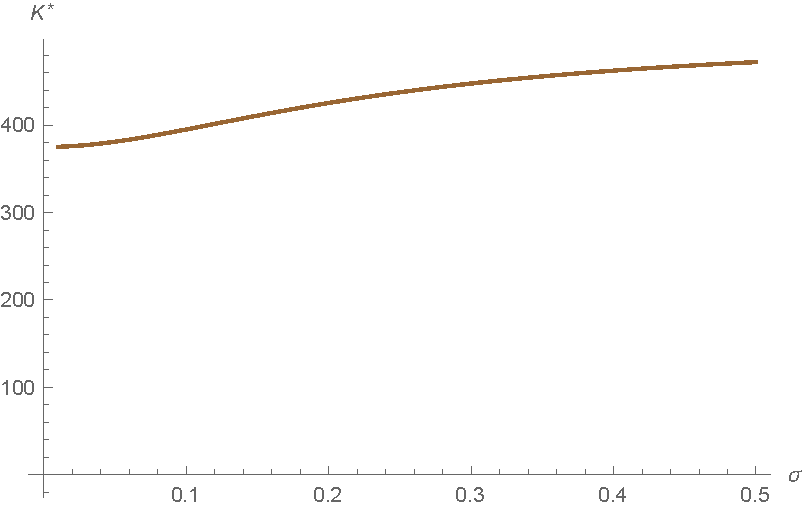
\includegraphics[width=0.32\textwidth]{StopTime/1_k.pdf}}
%	\end{subfigmatrix}
%	\caption{Sensibility analysis of the (estimated) mean of optimal investment time, the threshold level and the optimal capacity level (referred on Chapter \ref{chapter:1}) with the volatility, regarding different initial values $x_0 \in \{0.001, \ 0.01\}$.}
%	\label{fig:vol_1}
%\end{figure}
%
%Besides previous conclusions, on Table \ref{tab:vol_1}, we observe that the difference between $\tau_B^*$ and $\tau_C^*$, for $x_0=0.01$, is more noticeable than what it seems in Figure \ref{fig:vol_1}.
%
%We found no relation between the behaviour of optimal investing times and threshold levels or optimal capacity. However it seems to exist an optimal volatility level such that the optimal investment time is the lowest. In this case, this optimal volatility level $\sigma^*$ seems to be $0.15 < \sigma^* < 0.25$ for $x_0=0.001$ and $\sigma^*<0.15$ for $x_0=0.01$.
%
%\textcolor{red}{Referir esta parte do nível optimal de volatilidade? É verdade que a empresa não tem controlo sobre a volatilidade do nível de procura, contudo poderá escolher entre mercados com diferentes níveis de volatilidade. Mesma pergunta para todas as análises de volatilidade.}
%
%\textcolor{red}{Manter tabela?}
%
%\begin{table}[!ht]
%	\centering
%	\caption{Sensibility analysis of the (estimated) mean of optimal investment time, the threshold level and the optimal capacity level (referred on Chapter \ref{chapter:1}) with the volatility, regarding different initial values $x_0 \in \{0.001, \ 0.01\}$.}
%	\begin{tabular}{c|ccccccccl}
%		\hline
%		\text{ $\sigma $ } & 0.05 & 0.1 & 0.15 & 0.2 & 0.25 & 0.3 & 0.35 & 0.4 \\ \hline
%		$K^*$ & 381.04 & 395.08 & 410.92 & 425.39 & 437.62 & 447.66 & 455.80 & 462.41 \\
%		$x_B^*$ & 0.012 & 0.013 & 0.015 & 0.017 & 0.020 & 0.023 & 0.027 & 0.032 \\
%		$x_C^*$ & 0.017 & 0.019 & 0.022 & 0.027 & 0.032 & 0.038 & 0.045 & 0.053 \\ \hline
%	   $\overline{\tau _B}$ & 67.64 & 58.71 & 53.64 & 52.22 & 52.46 & 57.49 & 63.97 & 106.98 & \rdelim\}{2}{0.05mm}[$x_0=0.001$]  \\
%		$\overline{\tau _C}$ & 78.21 & 68.43 & 63.82 & 63.94 & 65.55 & 70.66 & 90.09 & 193.65 \\ \hline
%		$\overline{\tau _B}$ & 4.29 & 5.26 & 6.48 & 7.81 & 9.53 & 10.25 & 11.90 & 14.154 &	\rdelim\}{2}{0.05mm}[$x_0=0.01$] \\
%		$\overline{\tau _C}$ & 13.88 & 12.89 & 13.40 & 14.92 & 15.53 & 16.93 & 19.77 & 23.11
%	 \\ \hline
%	\end{tabular}
%\label{tab:vol_1}
%\end{table}
%
%
%Regarding the observed variation of considered parameters, on Figure \ref{fig:var_1}, we verify what was already stated. 
%For volatility values bigger than 0.35, we observe changes up to 140\% on the variation of optimal investment times' mean, making the growth of all other parameters to seem despicable, as can be seen in the leftmost side. 
%However when we focus on volatility values smaller than 0.35, the mean of optimal investment times doesn't vary significantly, having a variation in magnitude smaller than 4\%, as can be seen in the rightmost side.
%
%
%
%\begin{figure}[!ht]
%	\begin{subfigmatrix}{2}
%		\subfigure[Variation of parameters of interest for volatilities $\sigma \in (0,0.5)$. ]{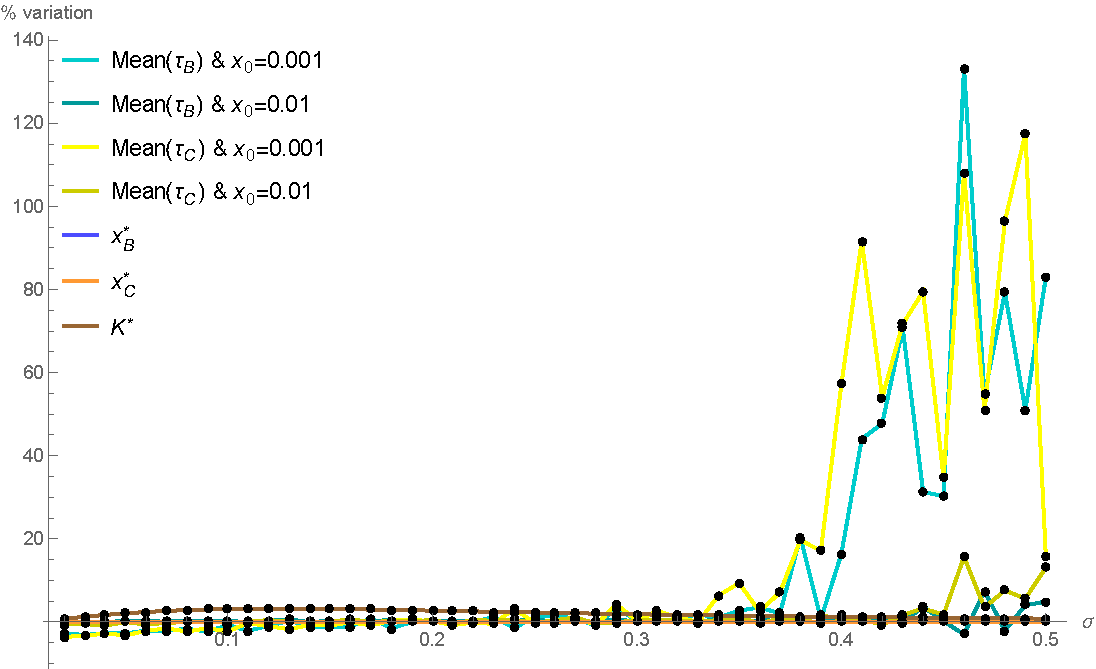
\includegraphics[width=0.4\textwidth]{StopTime/1_varSP500H1500.pdf}}
%		\subfigure[Variation of parameters of interest for volatilities $\sigma \in (0,0.35)$. ]{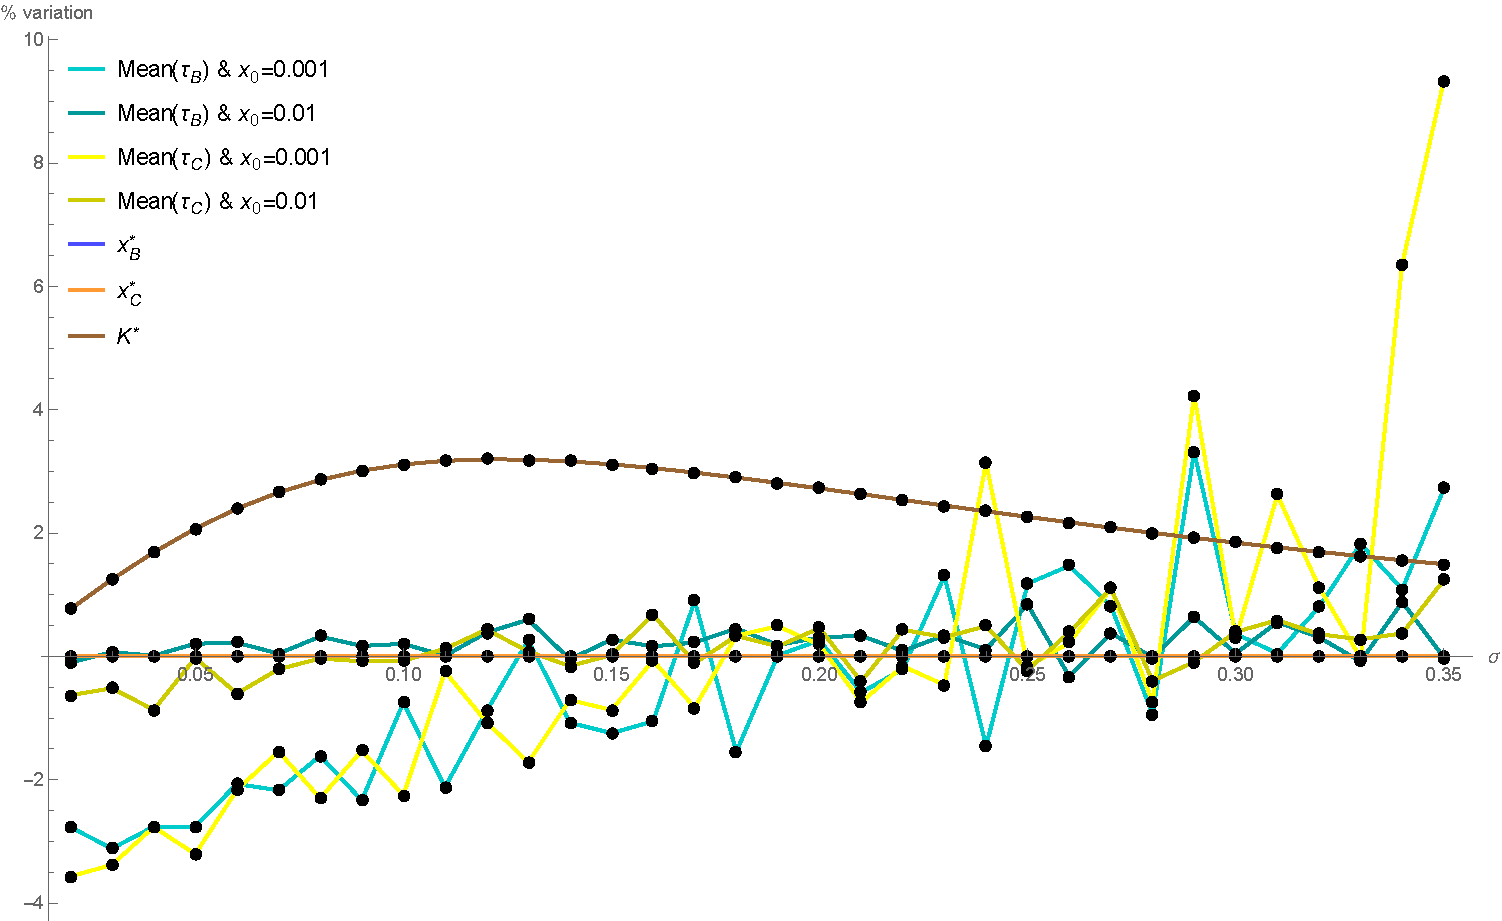
\includegraphics[width=0.4\textwidth]{StopTime/1_varSP500H1500_35.pdf}}
%	\end{subfigmatrix}
%	\caption{Variation of (estimated) mean of optimal investment time, the threshold level and the optimal capacity level (referred on Chapter \ref{chapter:1}) with the volatility, regarding different initial values $x_0 \in \{0.001, \ 0.01\}$.}
%	\label{fig:var_1}
%\end{figure}
%
%
%
%
%\vspace{3mm}
%$\bullet$ \textbf{Situation on Section \ref{chapter:2}: firm has an established product and want to introduce a new one, replacing the other one}
%
%
%On Figure \ref{fig:vol_2} we can observe that conclusions stated before hold. Optimal investment times have a non-monotonic behaviour with the volatility and they seem not to be related neither with threshold values or the optimal capacity level. 
%
%\begin{figure}[!ht]
%	\begin{subfigmatrix}{3}
%		\subfigure[(Estimated) mean of optimal investment times. ]{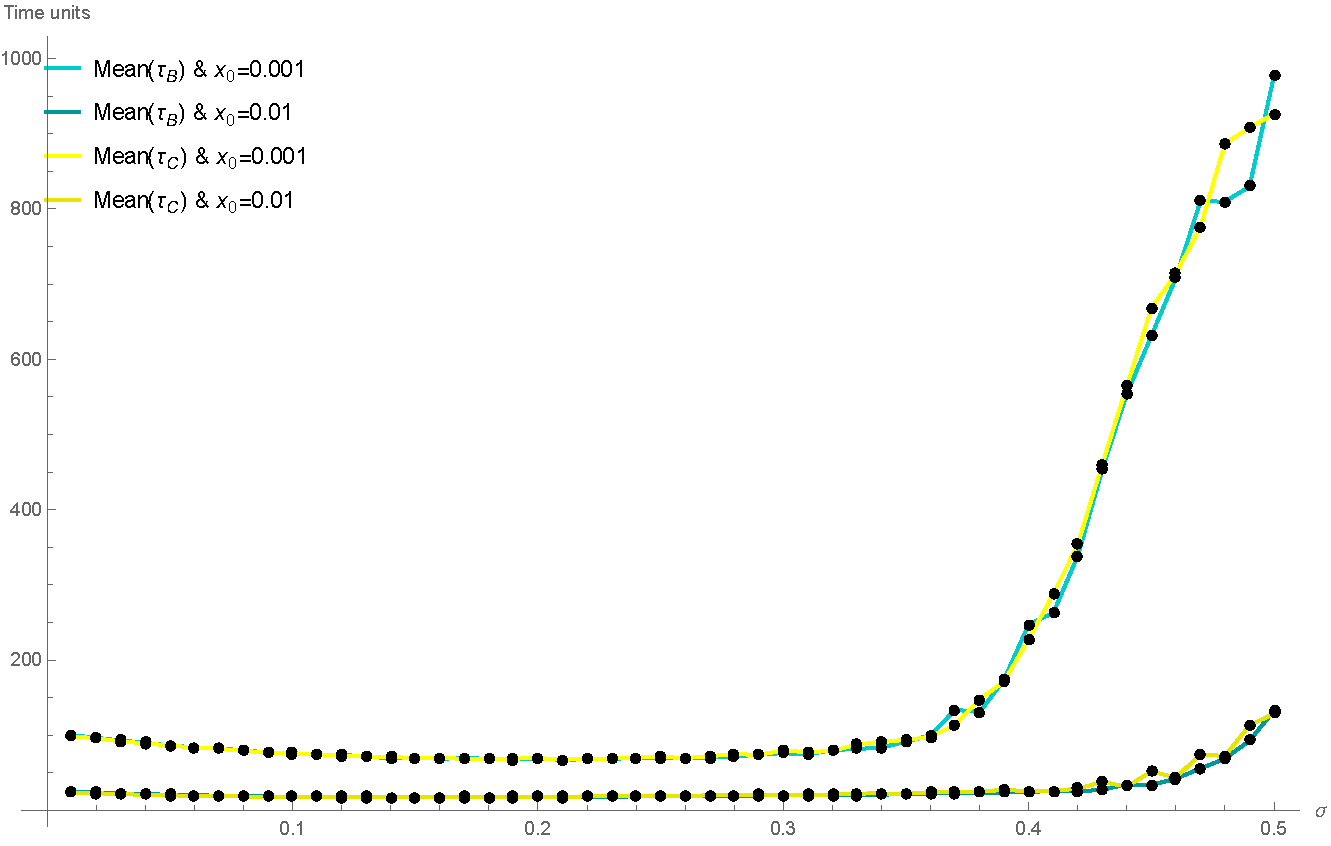
\includegraphics[width=0.32\textwidth]{StopTime/2_meantauSP500H1500.pdf}}
%		\subfigure[Demand threshold. ]{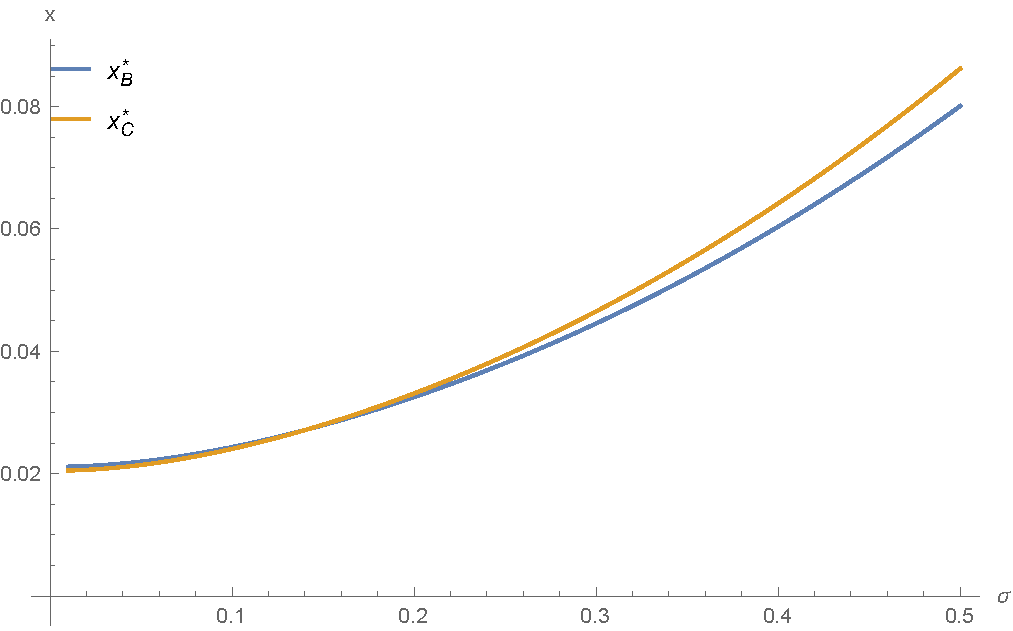
\includegraphics[width=0.32\textwidth]{StopTime/2_x.pdf}}
%		\subfigure[Optimal capacity level.]{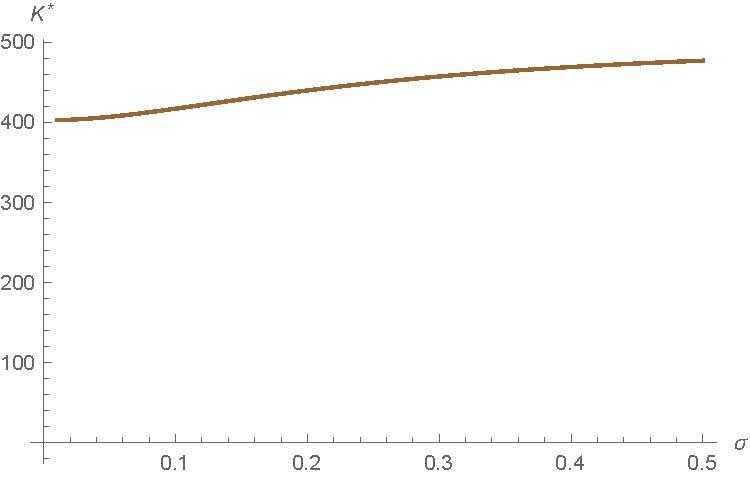
\includegraphics[width=0.32\textwidth]{StopTime/2_k.pdf}}
%	\end{subfigmatrix}
%	\caption{Sensibility analysis of the (estimated) mean of optimal investment time, the threshold level and the optimal capacity level (referred on Chapter \ref{chapter:2}) with the volatility, regarding different initial values $x_0 \in \{0.001, \ 0.01\}$.}
%	\label{fig:vol_2}
%\end{figure}
%
%Once again, confronting the results on Figure \ref{fig:vol_2} with the ones presented on Table \ref{tab:vol_2}, we observe that the idea of having an optimal volatility level might be also valid again.  In this case, the optimal volatility level $\sigma^*$ seems to be $0.15 < \sigma^* < 0.25$ for both initial values $x_0=0.001$ and $x_0=0.01$.
%
%
%\begin{table}[!ht]
%	\centering
%	\caption{Sensibility analysis of the (estimated) mean of optimal investment time, the threshold level and the optimal capacity level (referred on Chapter \ref{chapter:2}) with the volatility, regarding different initial values $x_0 \in \{0.001, \ 0.01\}$.}
%	\begin{tabular}{c|ccccccccl}
%		\hline
%		\text{ $\sigma $ } & 0.05 & 0.1 & 0.15 & 0.2 & 0.25 & 0.3 & 0.35 & 0.4 \\ \hline
%		$K^*$ & 406.62 & 416.81 & 428.59 & 439.60 & 449.10 & 457.01 & 463.51 & 468.84  \\
%		$x_B^*$ & 0.022 & 0.024 & 0.028 & 0.033 & 0.038 & 0.045 & 0.052 & 0.060  \\
%		$x_C^*$ & 0.021 & 0.024 & 0.028 & 0.033 & 0.039 & 0.047 & 0.055 & 0.064 \\ \hline
%		$\overline{\tau _B}$ & 86.86 & 76.4 & 71.57 & 65.01 & 68.18 & 73.59 & 84.79 & 203.85  & \rdelim\}{2}{0.05mm}[$x_0=0.001$]  \\
%		$\overline{\tau _C}$ & 86.45 & 75.33 & 69.36 & 67.75 & 71.57 & 76.08 & 99.44 & 194.35 \\ \hline
%		$\overline{\tau _B}$ & 20.94 & 18.04 & 18.04 & 17.19 & 17.37 & 19.55 & 22.19 & 25.88  &	\rdelim\}{2}{0.05mm}[$x_0=0.01$] \\
%		$\overline{\tau _C}$ & 20.34 & 18.69 & 18.18 & 17.94 & 19.88 & 21.21 & 22.04 & 23.02  \\ \hline
%	\end{tabular}
%\label{tab:vol_2}
%\end{table}
%
%
%Regarding the observed variation of considered parameters, on Figure \ref{fig:var_2}, we find a similar situation to the one described above.
%This time, the mean of optimal investment times vary up to 160\%  for volatility values bigger than 0.35, and vary up to 4\%, for volatility values smaller than 0.35.
%
%
%\begin{figure}[!ht]
%	\begin{subfigmatrix}{2}
%		\subfigure[Variation of parameters of interest for volatilities $\sigma \in (0,0.5)$. ]{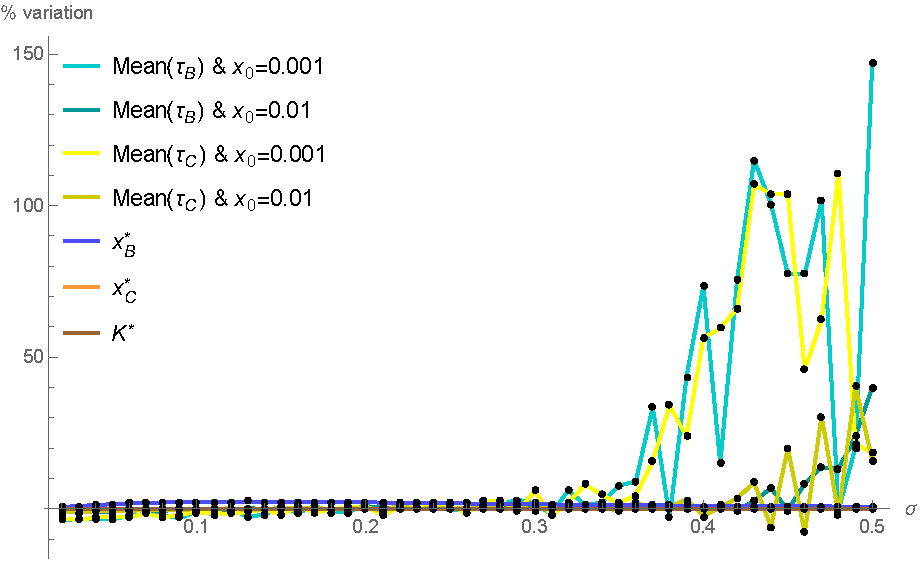
\includegraphics[width=0.4\textwidth]{StopTime/2_varSP500H1500.pdf}}
%		\subfigure[Variation of parameters of interest for volatilities $\sigma \in (0,0.35)$. ]{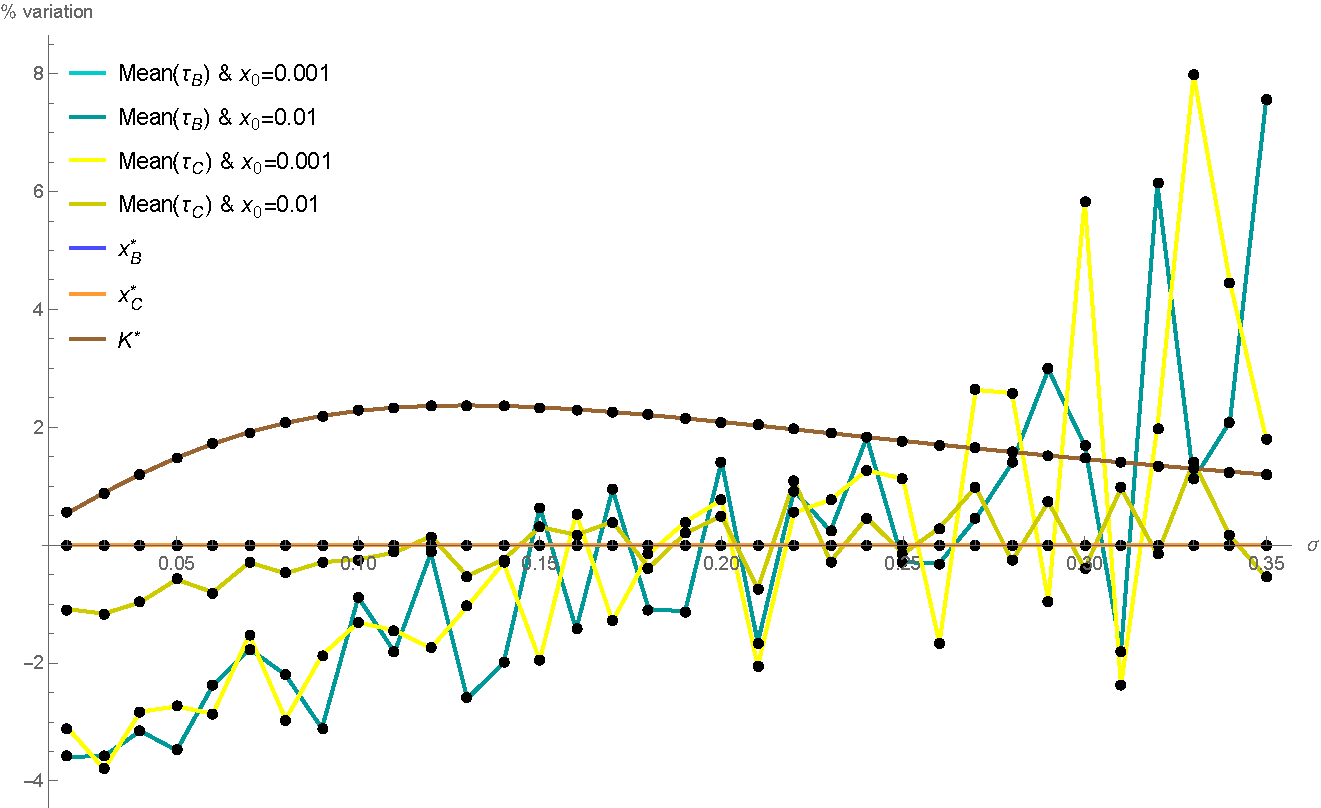
\includegraphics[width=0.4\textwidth]{StopTime/2_varSP500H1500_35.pdf}}
%	\end{subfigmatrix}
%	\caption{Variation of (estimated) mean of optimal investment time, the threshold level and the optimal capacity level (referred on Chapter \ref{chapter:2}) with the volatility, regarding different initial values $x_0 \in \{0.001, \ 0.01\}$.}
%	\label{fig:var_2}
%\end{figure}
%
%
%
%\vspace{3mm}
%$\bullet$ \textbf{Situation on Chapter \ref{chapter:3}: firm has an established product and want to introduce a new one, allowing a phase of simultaneous production}
%
%
%On Figure \ref{fig:vol_3}, there are represented both estimated means of optimal investment times upon which the firm should invest in the new product and start the simultaneous production of the old and new products, given initial demand values $x_0 \in \{ 0.001, \ 0.01 \}$, and the estimated mean of optimal time to suppress the production of the old product and start solely to produce the new product, considering the starting demand value to be $x_{1,A}^*$. We observe that this time none of the estimated means seem to vary significantly with the volatility level considered.
%
%
%\begin{figure}[!ht]
%	\begin{subfigmatrix}{3}
%		\subfigure[(Estimated) mean of optimal investment times.]{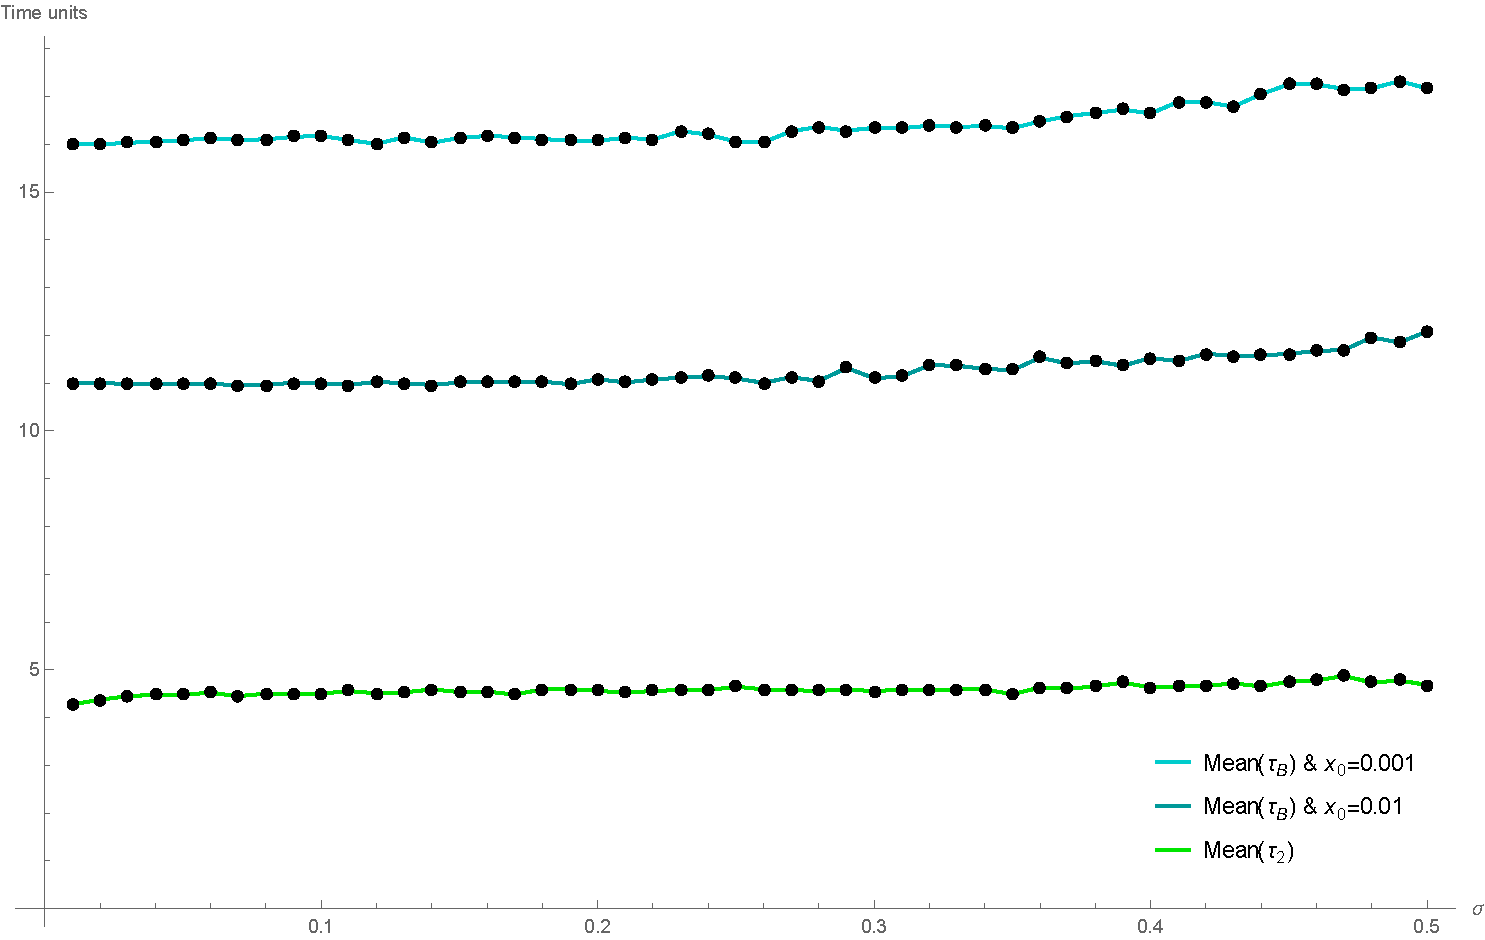
\includegraphics[width=0.32\textwidth]{StopTime/3_meantau.pdf}}
%		\subfigure[Demand threshold.]{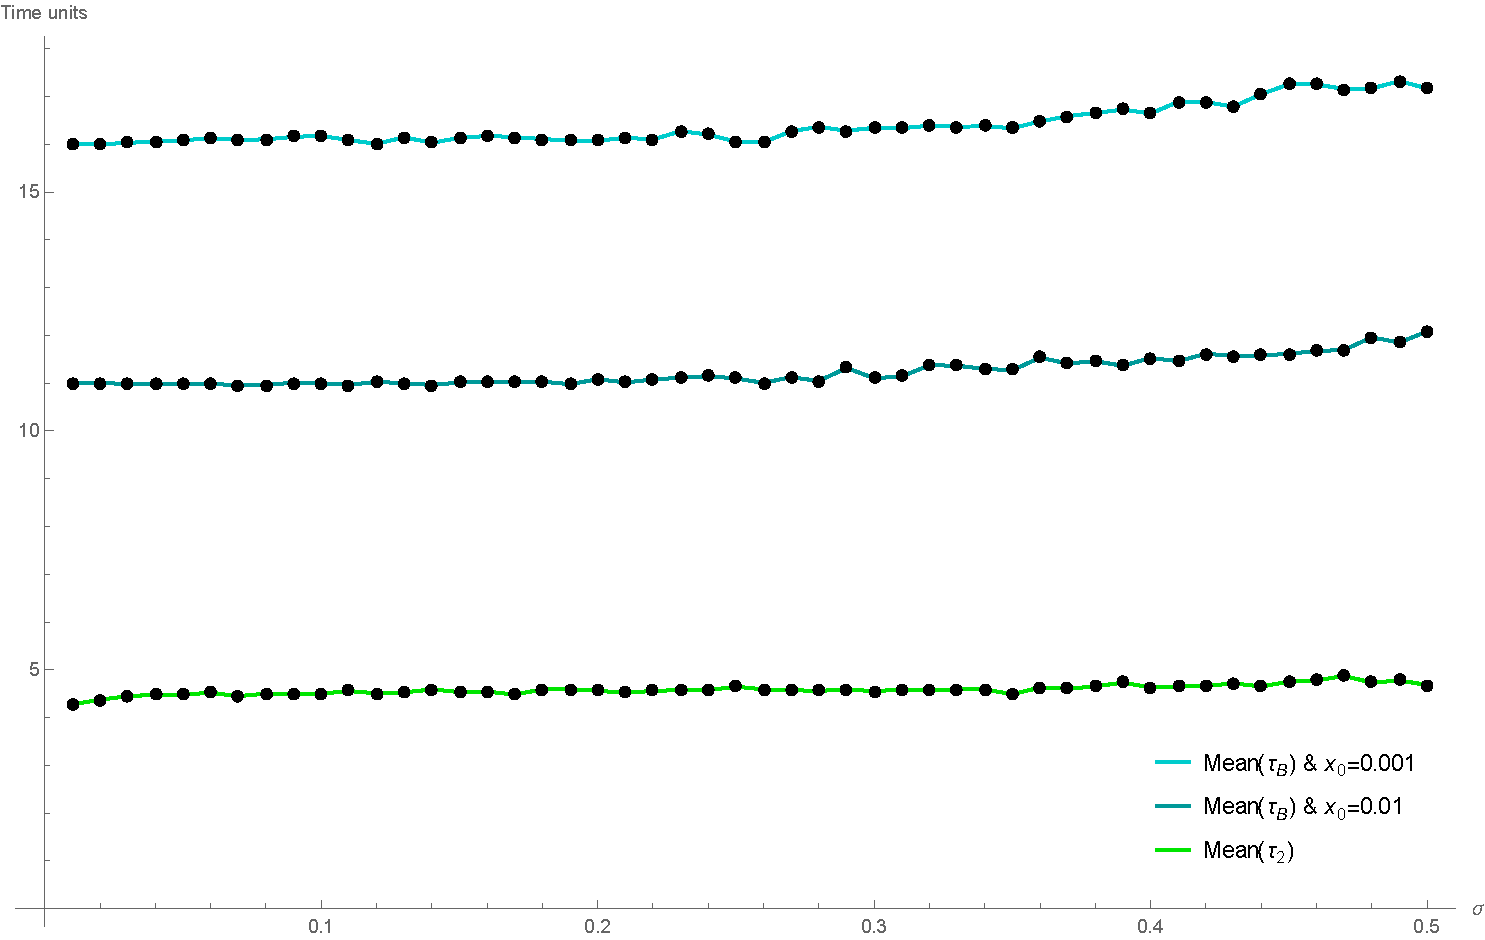
\includegraphics[width=0.32\textwidth]{StopTime/3_x.pdf}}
%		\subfigure[Variation of parameters of interest for volatilities $\sigma \in (0,0.5)$.]{\includegraphics[width=0.32\textwidth]{StopTime/3_var.pdf}}
%	\end{subfigmatrix}
%	\caption{Sensibility analysis of the (estimated) mean of optimal investment time, the threshold level and the optimal capacity level (referred on Chapter \ref{chapter:3}) with the volatility, regarding different initial values $x_0 \in \{0.001, \ 0.01\}$.}
%	\label{fig:vol_3}
%\end{figure}
%
%Confronting both results present on Figure \ref{fig:vol_3} and Table \ref{tab:vol_3}, we note that none of the estimated means seem to vary with the value of the correspondent threshold level for any level of volatility considered. In this situation, there is no evidence of an optimal volatility level that evidences a minimum investment time, as it happened in previous analysis.
%
%
%\begin{table}[!ht]
%	\centering
%	\caption{Sensibility analysis of the (estimated) mean of optimal investment time, the threshold level and the optimal capacity level (referred on Chapter \ref{chapter:3}) with the volatility, regarding different initial values $x_0 \in \{0.001, \ 0.01\}$.}
%	\begin{tabular}{c|ccccccccc}
%		\hline
%		\text{ $\sigma $ } & 0.05 & 0.1 & 0.15 & 0.2 & 0.25 & 0.3 & 0.35 & 0.4 \\ \hline
%		$x_{1,A}^*$ & 1.092 & 1.101 & 1.116 & 1.136 & 1.161 & 1.190 & 1.224 & 1.261   \\
%		$x_2^*$ & 6.518 & 6.572 & 6.659 & 6.779 & 6.928 & 7.104 & 7.306 & 7.530  \\ \hline
%		$\overline{\tau _{1,A}}$ & 16.08 & 16.18 & 16.13 & 16.07 & 16.06 & 16.34 & 16.34 & 16.64  & \rdelim\}{1}{0.05mm}[$x_0=0.001$] \\
%		$\overline{\tau _{1,A}}$ & 10.92 & 11.00 & 11.01 &  11.08 & 11.10 & 1.10 & 11.27 & 11.53 & \rdelim\}{1}{0.05mm}[$x_0=0.001$]  \\ \hline
%		$\overline{\tau _2}$ & 4.48 & 4.50 & 4.54 & 4.56 & 4.65 & 4.55 & 4.49 & 4.63   \\ \hline
%	\end{tabular}
%\label{tab:vol_3}
%\end{table}
%
%
%
%
%
%\vspace{3mm}
% We also performed simulations considering larger values of \texttt{NsamplePaths} and \texttt{horizon}. However we concluded that the precision of obtained results don't compensate the (considerable) raise on computational running time.
% 
% 
%\vspace{1cm}
%
%\textcolor{red}{Creio que este capítulo tem muita informação não explorada a fundo. Contudo não sei o que vale a pena mencionar sem estar a repetir o que já foi dito nas secções de Comparative Statics}